%This is the main document, translate only this one!
%All other .tex files are just subfiles of this shell and do not contain "\begin{document} ... \end{document}"
%If Czech characters do not translate in pdf correctly, go back to http://latex.feec.vutbr.cz/cz/latex/lokalni-instalace/instalace-miktex/ for proper activation of Czech support in MikTeX 

\documentclass{article}
\usepackage[T1]{fontenc}
%\usepackage[round]{natbib}
\usepackage[autostyle]{csquotes}



\usepackage[
    backend=biber,
    style=authoryear,
    natbib=true,
   % sortlocale=en_US,
    url=false, 
    doi=true,
    eprint=false,
    issn=false,
    isbn=false,
    maxcitenames=2,
    maxbibnames=99,
    uniquelist=false
]{biblatex}
%\DeclareLanguageMapping{english}{english-apa}

\AtEveryBibitem{%
  \clearlist{language}%
}
\addbibresource{bibliography.bib}


\makeatletter
% new code


\makeatother

\usepackage{bbm}

\usepackage[colorlinks=true, allcolors=blue]{hyperref}
\usepackage{graphicx}
\usepackage{enumitem}
\usepackage{booktabs}
%\usepackage{breqn}
\usepackage[flushleft]{threeparttable}
\usepackage{subcaption}
\usepackage{caption}
\usepackage{pdflscape}
\usepackage{longtable}
 \usepackage{array}
\usepackage{multirow}
   \usepackage[table]{xcolor}
   \usepackage{wrapfig}
   \usepackage{float}
   \usepackage{colortbl}
   \usepackage{tabu}
   \usepackage{threeparttablex}
   \usepackage[normalem]{ulem}
  \usepackage{makecell}
\usepackage{multirow}
\usepackage{setspace}
%\usepackage{bibentry}





\usepackage{url}
\usepackage[utf8]{inputenc}
%\usepackage{csquotes}
\usepackage[english]{babel}
\usepackage{amsmath}
\usepackage{color}
%\bibliographystyle{dcu}
% agsm, apacite, dcu

%\usepackage[a-2u]{pdfx}

\renewcommand{\baselinestretch}{1.5} 
\hoffset -1.54cm \voffset -0.04pt \evensidemargin 1.5cm
\oddsidemargin 2.5cm \topmargin -1.6cm
%% Vyska textu 232 mm
%% Sirka textu 136 mm
\textheight 232mm \textwidth 136mm

\newcommand{\noop}[1]{} 
%this should generate norm page of approx 1800 characters per page
%with 30 lines times 60 characters per line (excluding space)

\begin{document}
%\nobibliography*
\pagestyle{empty}
\begin{center}
%\textcolor{red}{[desky]} \\
\textbf{\LARGE{CHARLES UNIVERSITY IN PRAGUE}}\\
\Large{FACULTY OF SOCIAL SCIENCES}\\
\large{Institute of Economic Studies} \\
\vspace{60mm} \textbf{\LARGE{Bachelor thesis}}\\
\end{center}
\vspace{100mm} \textbf{\LARGE{2019}}  \hspace {65mm} \textbf{\LARGE{Martin Kosík}}\\
\vspace{11mm}
\newpage

\pagestyle{empty}
\begin{center}
\textbf{\LARGE{CHARLES UNIVERSITY IN PRAGUE}}\\
\Large{FACULTY OF SOCIAL SCIENCES}\\
\large{Institute of Economic Studies} \\
\scalebox{0.5}{

\includegraphics{LaTex/Title/karel.jpg}}\\  %you can choose karel.jpg, karelI.jpg or karelII.jpg
\textbf{\large{Martin Kosík
}} \\
\vspace{10mm} \textbf{\LARGE{Cultural norms and son preference }\\
 \LARGE{in developing countries}}\\
\vspace{11mm} \textit{\Large{Bachelor thesis}} \\
\vspace{40mm} \large{Prague 2019}

\end{center}
\newpage


\pagestyle{empty}

\vfill

\vglue 16cm

\noindent \large{Author: \textbf{Martin Kosík }}\\
\noindent \large{Supervisor: \textbf{doc. PhDr. Julie Chytilová, Ph.D.}}\\
\noindent \large{Reviewer: \textbf{}}\\
\noindent \large{Date of defense:}
\normalsize{\textbf{\textcolor{red}{[insert the year of defense]}}}\\
\newline
\noindent \large{Grade:} \normalsize{\textbf{\textcolor{red}{[insert the final grade]}}}\\

 %this just pastes here the content of "titlepage.tex" during LaTeX/PDF LaTeX/PDF TeXify translatation
\pagestyle{empty}

\section*{Bibliographic note}

\noindent KOVANDA, Karel. \textit{Nazev prace.} Praha 2010. 75 s.
Diplomov? pr?ce (Mgr.) Univerzita Karlova, Fakulta soci?ln?ch v?d,
Institut komunika?n?ch studi? a ?urnalistiky. Katedra medi?ln?ch
studi?. Vedouc? diplomov? pr?ce Prof. PhDr. Jan Nov?k, CSc. \\
\textbf{\textcolor{red}{[p?i tvorb? bibliografick?ch citac?
vych?zejte z normy ?SN ISO 690, ?SN ISO 690-2 nebo podle jin?ch
doporu?en?ch cita?n?ch styl?]}}\\

\section*{Abstract}
  I study how geopolitical concerns influence attitudes of a state toward its minorities. I exploit the  Hitler's rise to power in 1933 as an exogenous shock to Soviet-German relations. 
    Using the digitized archival data on 2.7 million individual arrests by the Soviet secret police, I apply difference-in-differences and synthetic control method to estimate how changing geopolitical relations influenced repressions of Germans in the USSR. The estimates of both models imply that that the arrests of Germans relative to other minorities increased by approximately 2\% after 1933. 

\section*{Keywords}
repression, geopolitics, Soviet Union, difference-in-differences, synthetic control method, \\
\newpage

\section*{Abstrakt}
Whoa. \\




\section*{Klíčová slova}
represe, geopolitika, Sovětský svaz, \\

\newpage
 %this just pastes here the content of "abstract.tex" during LaTeX/PDF LaTeX/PDF TeXify translatation
\pagestyle{empty}

\vfill

\vglue 12cm

\section*{Declaration of Authorship}
I hereby proclaim that I wrote my bachelor thesis on my own under
the leadership of my supervisor and that the references include all
resources and literature I have used.

\bigskip

\noindent I grant a permission to reproduce and to distribute copies
of this thesis document in whole or in part. \vspace{0.5cm}

\begin{table}[!hbp]
\begin{tabular}{lr}
\hspace{-0.3cm} Prague, \today \hspace{6.07cm}
 \begin{tabular}{p{3.57cm}} %3.7
    \vspace{0.6cm} \\ \\
     \hline \\ \vspace{-0.7cm} \hspace{1cm} Signature
 \end{tabular}

\end{tabular}
\end{table}


\newpage

\vfill

\vglue 15cm

\section*{Acknowledgment}
\noindent I would like to express my gratitude to ... 

 %this just pastes here the content of "declaration.tex" during LaTeX/PDF LaTeX/PDF TeXify translatation
\pagestyle{empty}
\begin{center}
\LARGE{The Bachelor’s Thesis Proposal}
%\LARGE{Master of Bachelor Thesis}
\end{center}
\vspace{5mm}
\begin{tabular}{lcl}
\large{\bf Schedule for the bachelor exam:} & & \\
\large{\bf Author of the bachelor thesis:} & & \large{\bf Martin Kosík}\\
\large{\bf Supervisor of the bachelor thesis:} & & \large{\bf Julie Chytilová}
\end{tabular}
\\
\\
\\
\begin{tabular}{lcl}
\large{\bf Theme:} & & \large{\bf The Geopolitics of Repressions}
\end{tabular}\\
\\
\\
\large{\bf Research question and motivation}
%\par

\noindent
What determines the attitude of a state toward ethnic minorities within its borders? Why are some minorities accommodated or assimilated and others are politically excluded and repressed? Furthermore, why does the position of a state toward its minorities change in time? 

\citet{mylonas_politics_2013} argues that geopolitical concerns play an important role. Specifically, a state is likely to choose repression and exclusion if the ethnic minority's country of origin is seen as a geopolitical enemy. The minority is then viewed by the state as unreliable and as a potential fifth column of the foreign country. 

I will test this hypothesis on the case of the German minority in the Soviet Union. In 1933, Hitler’s rise to power changed Germany from a neutral actor to an ideological and geopolitical enemy in the perspective of the Soviet Union. This enables us to estimate how the repression of Germans in the USSR changed before and after 1933 and compare it with other minorities. In particular, I plan to use the individual arrests by the Soviet secret police (NKVD) as a dependent variable and employ the difference-in-differences strategy. 

\noindent  \large{\bf Contribution}

\noindent Existing literature on repressions has focused mostly on their consequences and legacies (Rozenas, Schutte, and Zhukov 2017; Lupu and Peisakhin 2017; Zhukov and Talibova 2018). As far as the strategic use of repressions by the state is studied, it is usually in relation to domestic factors such as institutions and economic shocks (Davenport 2007; Greitens 2016; Blaydes 2018) with less attention being given to external forces. An exception to this is a study by Mylonas (2013) which tests his theory with data on the post-World War I Balkans. However, his cross-sectional regression might suffer from omitted variable bias and reverse causality and my approach hopefully offers cleaner identification. 

My bachelor thesis can also contribute to the literature on the origins of Soviet ethnic repressions. Although many scholars argue that a perceived connection to hostile external powers has played a role \citep{martin_origins_1998, polian_against_2003}, the evidence has been mostly qualitative and anecdotal. 

\noindent \large{\bf Methodology}

\noindent My main source of data will be replication files from \citet{zhukov_stalins_2018} who use lists of victims of Soviet political repressions aggregated by Russian NGO Memorial. The difference-in-differences strategy will be used to estimate the impact of change German-Soviet relations caused by Hitler’s rise to power on arrests of Germans in the USSR. 

However, the parallel trends assumption, which is necessary for unbiasedness of difference-in-differences, can in some cases be violated. As a robustness check, I plan to apply the synthetic control method which constructs a synthetic control group as a linear combination of untreated units (in our case ethnicities) based on matching of pre-treatment trends and time-invariant covariates %\citep{abadie_economic_2003, abadie_synthetic_2010}
(Abadie and Gardeazabal 2003; Abadie, Diamond, and Hainmueller 2010). 

\noindent \large{\bf  Outline}
\begin{enumerate}
\item Introduction
 \item Literature review 
 \item Historical background
 \item Data
 \item Methodology
 \item Results
 \item Conclusion 
\end{enumerate}
\medskip
\large{\bf References:}
%example of book reference
\printbibliography[keyword=major, heading=none]
%\bibentry{zhukov_stalins_2018}  \\

%\fullcite*{abadie_synthetic_2010} \\
%example of preprint reference
%\lbrack 2\rbrack \hspace{1pt} S. Leyffer, T. Munson (2005):Solving Multi-Leader-Follower
\vspace{15mm}\\
In Prague on ..........\newline \\
Signature of the supervisor \hspace{30mm} Signature of the author
 %this just pastes here the content of "project.tex" during LaTeX/PDF LaTeX/PDF TeXify translatation
% Note: "project.tex" no longer corresponds to the SIS output
\pagestyle{plain} \setcounter{page}{1} % "\setcounter{page}{xx}" changes the current page counter to a new value "xx"

\selectlanguage{english}
\title{The Geopolitics of Repressions}
\author{Martin Kosík}


\pagenumbering{roman}

%\maketitle

%\begin{abstract}  I study how geopolitical concerns influence attitudes of a state toward its minorities. I exploit the  Hitler's rise to power in 1933 as an exogenous shock to Soviet-German relations.  Using the digitized archival data on 2.7 million individual arrests by the Soviet secret police, I apply difference-in-differences and synthetic control method to estimate how changing geopolitical relations influenced repressions of Germans in the USSR. The estimates of both models imply that that the arrests of Germans relative to other minorities increased by approximately 2\% after 1933. \end{abstract}

\newpage
 \tableofcontents
\newpage
\pagenumbering{arabic}
%\pagestyle{headings}
%example of the text

\section*{Introduction}
\addcontentsline{toc}{section}{Introduction}
What determines the attitude of a state toward ethnic minorities within
its borders? Why are some minorities accommodated or assimilated and
others are politically excluded and repressed? Furthermore,  why does the
position of a state toward its minorities change in time? For example
Soviet Union largely accommodated its minorities by in 1920s but it
heavily repressed them in campaigns of mass terror 10 years later. 

%Some studies emphasize that certain domestic institution such as democracy can decrease the likelihood of persecutions. However this does not explain why the same states often treat its ethnic minorities so differently.  For example (give example, man)...\\
%\citet{mylonas_politics_2013} argues that geopolitical concerns play inportant role. Specifically, the state is likely to choose repression and exclusion against a minority group if a external power with ethnic ties to the group is a geopolitical enemy.  
\citet{mylonas_politics_2013} argues that geopolitical concerns play an important role. Specifically, a state is likely to choose repression and
exclusion if the ethnic minority's country of origin is seen as an
geopolitical enemy. The minority is then viewed by the state as
unreliable and as a potential fifth column of the foreign country.   

We test this hypothesis on the case of German minority in Soviet union.
In 1933, Hitlers rise to power changed Germany from a neutral actor to ideological and geopolitical enemy in the perspective of the Soviet Union. We can then see how the repression changed before and after 1933 and compare it with other minorities. In particular, we use the individual arrests by soviet secret police (NKVD) as a dependent variable and employ the difference in difference strategy. 

%First, the Soviet Union was large multiethnic state whose attitude to its minorities drastically changed throughout the year with   

%We use the case of German minority in the Soviet Union to test this hypothesis for several reason.  

%We test hypothesis put forward by Mylonas (2012) according to which the host state is likely to choose repression and exclusion if the ethnic minority's country of origin is seen as geopolitical enemy. 


%We test this hypothesis on the case of German minority in Soviet using the rise of Hitler as a change of geopolitical relations. 


\entryneedsurl{ferman_cherry_2018}
\entryneedsurl{kaul_synthetic_2018}
\entryneedsurl{frierson_russias_2014}

\newpage
\section{Literature Review} \label{sec:lit_rev}
%The existing literature on the use of repression by a state have mostly focused on the impact of  of domestic factors such as institutions and economic growth \citep{davenport_state_2007-1}.
Existing literature on repressions has focused mostly on their consequences and legacies \citep{rozenas_political_2017, lupu_legacy_2017, zhukov_stalins_2018}. As far as the strategic use of repressions by the state is studied, it is usually in relation to domestic factors such as institutions and economic shocks \citep{davenport_state_2007-1, greitens_dictators_2016, blaydes_state_2018} with less attention being given to external forces. 

\citet{davenport_state_2007-1} finds that democracy is correlated with lower levels of repression. However, it is mainly free electoral competition rather than constraints on power of the executive that accounts for this negative effect.  
\citet{greitens_dictators_2016} links the severity of repression to the threat from dictator's inner circle. A dictator who fears that he would be deposed in a coup rather than in popular uprising will fragment their coercive apparatus in order to weaken the power of a potential challenger from within. The weakened secret police will be, according to Greitens, more likely to use violence since it fails to identify the transgressors and cannot effectively deter dissent. 
Other scholars see repression as a substitute for co-option \citep{wintrobe_political_1998, svolik_politics_2012}. Instead relying on the threat of persecution, an authoritarian ruler might buy the loyalty of the population by distributing rents to the supporters of the regime usually through the party apparatus. Negative economic shocks can then increase repression since the rents are no longer available.  \citet{blaydes_state_2018} 
illustrates this on the case of Iraq under Hussein where lower oil prices 

Furthermore, \citet{blaydes_state_2018} presents a theory attempting to explain different levels of repression across ethnic minorities within a country. She argues that the nature of repression  depends on the legibility of the ethnic group to the state.\footnote{The term legibility in this context means ability of a state to identify individuals in a given population and gather information on them.}
%(i.e. ability to gather information on its population) 
 Since the state coercive institutions cannot reliably identify transgressors in  less legible population (because of, for example, greater cultural and linguistic distance), they will more tend to resort to collective punishment. The logic behind this is that the members of the group will police its members to avoid collective punishment. 
%argues that repression can be a subsitute for economic rents.  

Our research also contributes to the literature studying factors that influence position of a state towards its ethnic minorities and under what conditions conflict is likely to occur. Size and and distribution of ethnic groups have been emphasized. Several scholars pointed out that
states with large number of ethnic groups are more likely to violently repress calls for autonomy or secession to discourage other ethnic minorities from making similar demands in the future \citep{evera_hypotheses_1994, toft_geography_2005,walter_reputation_2009}. 
% On the other hand, binational countries such as former Czechoslovakia  
Furthermore,  \citet{toft_geography_2005} argues that geographically concentrated groups tend to view their ethnic homeland as indivisible and non-negotiable issue which increases the likelihood of violent conflict. However, these approaches fail to explain changes in state's attitudes to minorities over short periods of time when the size and distribution of ethnic groups remains roughly constant. 
% možná tam hoď Votes and Violence od Wiliknsona

More recently, the role of international factors have received greater attention.  \citet{butt_secession_2017}  argues that response of a state to a secessionist movement depends on external security environment and outside actors. Specifically, a state located in a war-prone region is more likely to suppress demands for secession because loss of territory and population would make it vulnerable  to a potential future attack. Furthermore, a state responds with more violence if a separatist movement receives a support from an external power since the outside assistance makes the secessionists stronger. In addition to these strategic reasons, Butt emphasizes that  receiving external support incites  a strong feeling of betrayal to the central state.   
%\citet{svolik_politics_2012} sees repression as one of the tools of the authorian regime to keep conrol. Co-option and repression. Whereas the co-option is costly, repression requires greater power to the military. This might theaten the dictator's rule. However, this does not address different levels of repressions applied to different ethnic groups. 

As was mentioned, \citet{mylonas_politics_2013} puts forward a theory explaining how geopolitical relations influence the attitude of a state towards its minorities. The model features an ethnic minority living within a host state and  an external power. Moreover, Mylonas distinguishes between hosts states with revisionist foreign policy which want change the international status quo (e.g. because they gained power or lost territory in the past) and host states that prefer the current international order. 

The predictions of the theory are summarized in the table \ref{tab:mylonas}. First, if a minority group is not supported by any external power, the theory predicts that the host state will pursue policy of assimilation towards the group to \enquote{immunize} it from possible future  agitation  of external powers. Second, if an ethnic minority is supported by geopolitical ally then accommodation is likely since more repressive policies towards the minority could jeopardize the alliance. Third, theory predicts assimilation if a minority is supported by an geopolitical enemy and a host state pursues non-revisionist foreign policy because exclusionary policies could trigger new hostilities threatening the status quo. 
Finally, support of an external enemy combined with revisionist foreign policy will likely lead to exclusion of a given ethnic group since it is view as a potential \enquote{fifth column} of the external power. 

% Please add the following required packages to your document preamble:
% \usepackage{multirow}

\begin{table}[]
{\setstretch{2}
\begin{tabular}{llccc}
                                                                                                                     &                                           & \multicolumn{3}{c}{\textbf{External Power Support}}                                                                           \\ \cline{3-5} 
                                                                                                                     & \multicolumn{1}{l|}{}                     & \multicolumn{2}{c|}{\textbf{Yes}}                                        & \multicolumn{1}{c|}{\textbf{No}}                   \\ \cline{3-5} 
                                                                                                                     & \multicolumn{1}{l|}{}                     & \multicolumn{2}{c|}{Interstate Relations}                                & \multicolumn{1}{c|}{\multirow{4}{*}{Assimilation}} \\ \cline{3-4}
                                                                                                                     & \multicolumn{1}{l|}{}                     & \multicolumn{1}{c|}{\textbf{Ally}} & \multicolumn{1}{c|}{\textbf{Enemy}} & \multicolumn{1}{c|}{}                              \\ \cline{2-4}
\multicolumn{1}{l|}{\multirow{2}{*}{\textbf{\begin{tabular}[c]{@{}l@{}}Host's State\\ Foreign Policy\end{tabular}}}} & \multicolumn{1}{l|}{\textbf{Revisionist}} & \multicolumn{1}{c|}{Accommodation} & \multicolumn{1}{c|}{Exclusion}      & \multicolumn{1}{c|}{}                              \\ \cline{2-4}
\multicolumn{1}{l|}{}                                                                                                & \multicolumn{1}{l|}{\textbf{Status Quo}}  & \multicolumn{1}{c|}{Accommodation} & \multicolumn{1}{c|}{Assimilation}   & \multicolumn{1}{c|}{}                              \\ \cline{2-5} 
\end{tabular}
\caption{\label{tab:mylonas}Theoretical predictions of \citet{mylonas_politics_2013}}
\centering}
\end{table}


We can apply the theory to our case. First, the Soviet Union was arguably a revisionist state. The Bolsheviks had to accept large losses of territory under the Treaty of Brest-Litovsk in 1918 so that they could focus on fighting in Russian Civil War. Thus, the USSR would certainly prefer to change the international status quo. Second, the German-Soviet relations were neutral of even moderately friendly prior to 1933 but turned hostile after the rise of Hitler (described in greater detail in subsection \ref{subsec:relations}). Therefore the theory predicts that the policy 
of the Soviet state towards the German minority should change from accommodation to exclusion. \citet[p. 22]{mylonas_politics_2013} defines exclusion as \enquote{policies that aim at the physical removal of a non-core group from the host state.} The Soviet political repression which usually featured either outright execution or a term in a labor camp in the Far East of the country fits this description well. Thus, the theoretical expectation is that  repressions of Soviet Germans relative to other minorities should increase after 1933. 

Our main contribution is empirical test of this theory using a credible identification strategy. Most studies presented in this review test their hypotheses only by qualitative comparison of selected cases. Quantitative research usually involve only cross-sectional regressions based on categorical dependent variables.    

For example, \citet{mylonas_politics_2013} tests his theory with data on the post-World War I Balkans where the nation-building policies (categorized into 3 groups: accommodation, assimilation and exclusion)  toward  90 ethnic groups are a dependent variable and information on their support by external powers is an explanatory variables (together with other control variables). However, the results of the cross-sectional regression, used in the study, might easily be biased due to omitted variables or reverse causality and we believe that our approach offers cleaner identification.

%According to \citet{blaydes_state_2018}, a state will resort to collective punishment (based on ethnicity, religion or community membership) if it faces environment with highly asymmetric information in which it cannot identify the likely transgressors. The logic behind this is that the members of the community will police its members to avoid collective punishment. 


\citet{mcnamee_demographic_nodate} is methodologically and thematically closet study to ours. They analyze how the 1958 split in Soviet-China relations affected the demographic composition of the population in the Soviet-Chinese border regions.
Using difference-indifference strategy, they find that, after the split,  both states supported expulsions  of the minority group and sponsored immigration of the majority group but only in border regions without significant natural boundary (e.g. high mountains). They conclude that the states use demographic engineering as a way to protect their vulnerable border against a hostile power. 


%Hod tam koyamu, Zhurkavskayu a doten-snitken

\newpage
\section{Historical Background} \label{sec:hist_back}
%\subsection{German minority in the Soviet Union}
In this section, we provide brief historical context for selected topics. Specifically, we first describe  changing geopolitical relations of Germany and the Soviet from 1920 to 1941. In the next subsection, we provide brief overview of the most important aspects of Soviet political repression. Finally, evolution of the Soviet policy towards its ethnic minorities is summarized.   
\subsection{German–Soviet Relations in the Interwar Period} \label{subsec:relations}
The relations between Weimar Germany and Soviet Union can be characterized as neutral or even cooperative. Both countries were somewhat isolated in the international system dominated by the Western powers (Great Britain, France, USA) and sought to find allies. The good relations were first established by the Treaty of Rappalo in 1922 in which both countries renounced the territorial and financial claims against each other and agreed to secret military cooperation \citep{gatzke_russo-german_1958} and then reaffirmed by the Treaty of Berlin in 1926. Furthermore, a trade treaty was signed between the two countries in 1925 \citep{morgan_political_1963}.

Hitler was named chancellor on 30 January 1933 and effectively become a dictator on 24 March 1933 by the passing of the Enabling Act. 
The relations with Soviet Union quickly turned hostile for several reasons.  First, Hitler called in \emph{Main Kampf} for Germany to obtain \emph{Lebensraum} (living space) in the east, presumably at the expense of the Soviet Union and he often spoke of Judeo-Bolsheviks \citep[p. 6]{haslam_soviet_1984}. Moreover, Hitler's anti-communist was one of factors contributing to his political success as he presented himself as the only leader strong enough to  prevent a Communist revolution in Germany. This was not only empty rhetoric as he soon after his rise to power banned the German Communist Party and started to persecute its members \citep[chapter 5]{evans_coming_2004}. 

The opposition to fascism led to change in policy of the Communist International (Comintern)  with appointment Georgi Dimitrov as  its general secretary in 1934. The Communist parties in democratic countries were now encouraged to form coalitions (Popular Fronts) with social democratic parties to prevent rise of fascism, in contrast to the previous aggressive and uncompromising approach. This policy was affirmed by the Seventh World Congress of the Comintern in 1935 \citep{haslam_comintern_1979}.

The newly formed Popular Front coalitions won elections and entered government in some European countries including France and Spain. In Spain however, the coup of nationalists against the new government in 1936 sparked a civil war. The Soviet Union heavily supported the republican government, while Germany supplied the nationalists which further increased the tensions between the two countries. 
As a response to increasing tensions, Japan and Germany signed the Anti-Comintern Pact in 1936 in which they committed to  co-operate for defense against communistic disintegration. 
%Meanwhile in the Soviet Union, many people were persecuted for alleged cooperation with Germany including leading general Mikhail Tukhachevsky. 

The orientation of German foreign policy began to shift in spring of 1939.
Until that point, Hitler hoped that he could ally with Poland in a war against the Soviet Union or that Poland would at least allow the passing of German troops \citep[chapter 26]{weinberg_hitlers_2010}. 
%tried to court Poland to join the Anti-Comintern Pact against the Soviet Union 
But Poland repeatedly refused the German offers for closer relations such as to join the Anti-Comintern Pact and thus Hitler changed the strategy and  in April 1939 ordered the German army to began planing for the invasion of Poland \citep[p. 621]{kotkin_stalin:_2017}. However, France and Great Britain granted security guarantees to Poland in March 1939. 
Hitler thus tried to negotiate neutrality of the Soviet Union in war to avoid simultaneously facing  Western powers, Poland and the Soviet Union.
Soviet neutrality was potentially beneficial for Stalin too. A long and 
costly war would weaken the both the capitalist and fascist enemies of the 
Soviet Union. Moreover, Stalin believed that conditions of war could bring 
about socialist revolutions in those countries just as in Russia in 1917.  
After brief negotiations, on 23 August 1939   the  Molotov-Ribbentrop pact 
was signed between Germany and the USSR which guaranteed non-belligerence 
between the two countries. In addition,  a secret protocol of the treaty marked the German and Soviet spheres of influence in Eastern Europe.

%Therefore in case of war, Germany could be facing coalition of Western powers, Poland and the Soviet Union. 


%Nevertheless, the Soviet Union and Nazi Germany were able to cooperate inareas of common interest under special circumstances in late 1930s. Inparticular, on 23 August 1939 they sighed the  Molotov-Ribbentrop pact which guaranteed non-belligerence between Germany and the USSR and dividedthe spheres of influence in the Eastern Europe. This of course ended with German invasion into the USSR in June, 1941.  

%Except the brief period of limited cooperation, the Germany represented an ideological and geopolitical opponent. The Soviet propaganda portrayed Nazi
%Germany as an existential enemy and rank-and-file NKVD officers would
%perceive it as such (which is why Molotov-Ribbentrop pact caused such a surprise). \citep{kotkin_stalin:_2017}
The pact of the two former ideological enemies caused great shock and astonishment both among Party officials and ordinary people. 
Victor  \citet[p. 332]{kravchenko_i_1947}, a Soviet official who later defected to the US,   described in  his memoir the disbelief upon hearing about the pact  
\begin{quote}
There must be some mistake, I thought, and everyone around me seemed equally incredulous. After all, hatred of Nazism had been drummed into our minds year after year.  The big treason trials [...] have rested on assumption that Nazi Germany and its Axis friends [...]  were preparing to attack us. 
\end{quote}
Another party official later recalled that \enquote{it left us all stunned, bewildered, and groggy with disbelief} \citep[p. 137]{robinson_black_1988}. 

Nazi Germany attacked Poland on 1 September 1938 from the west and shortly after that, on 17 September, the Red Army invaded the eastern part of the country.  As was agreed in the pact, Poland was partitioned between Germany and the Soviet Union.
However, the mistrust between the two countries was still present as evidenced by a violent clash of German and Soviet troops near Lwów on 20 September.
%The pact, however, did last only 2 years and was marked by strong mutual distrust. 
%Other 

Hitler enjoyed major success in the first years of the war.
By summer 1940, German forces defeated French army and annexed Denmark and Norway. However, German industry was severely lacking raw materials needed in war effort against Britain and the US which, according to some historians, motivated Hitler to invade the resource-rich USSR \citep{tooze_wages_2008}. The German attack on the Soviet Union on 22 June 1941 ended 2 years of fragile cooperation.

The Eastern Front became the most bloody theater of World War II. 
It became the site of the worst atrocities including the Holocaust, starving of more than 3.3 million of Soviet prisoners of war and other.
\subsection{Soviet Political Repressions}
The Soviet Union had massive coercive apparatus. The Soviet secret police (which was throughout the years named the Cheka, OGPU, NKVD, MVD and  the KGB)\footnote{We will refer to the Soviet secret police as the NKVD in this text since this was the name of the agency for the largest part of the period of our interest} employed at its height (1937–1938)  270,730 persons \citep[p. 2]{gregory_terror_2009}. 
%The gulag  
The political repressions were usually carried under Article 58 of the Criminal Code. The Article 58 punished counter-revolutionary activities 
%defined as "any action aimed at overthrowing, undermining or weakening of the power of workers' and peasants' Soviets... and governments of the USSR". This 
which included treason, espionage, counterrevolutionary propaganda or agitation and  failure to report any of these crimes.  
In practice, this broad definition meant that anyone regarded as politically inconvenient could be arrested and prosecuted. 

During the mass operations, the central office of the NKVD would typically set quotas for the number of arrests which the regional branches were supposed to reach and exceed \citep[chapter 6]{gregory_terror_2009}. The local NKVD officer had to decide themselves who to target to meet the quotas. 

The sentences were in most cases issued extrajudicially by so-called \enquote{troikas}, three-person committees composed of a regional NKVD chief, a regional party leader, and a regional prosecutor. The NKVD chief usually dominated the process as party leaders sometimes feared that they themselves would be targeted \citep[p. 82]{snyder_bloodlands:_2011}. Only rarely was a person acquitted from his charge. 
% mozna napis neco o vyslichani jak je ve snyderovy na 82
The most common sentences for political crimes in the Stalinist period were  execution and prison term in a labor camp (Gulag) \citep[p. 21]{gregory_terror_2009}. 
A term in the Gulag of less then 5 years was considered lighter sentence in these cases.
% napis tady o Gulagech 

 With the rise in  repressions in the 1930s, the Gulag system significantly expanded. At its height, it consisted of at least 476 distinct camp complexes each containing hundreds of prisoners. The Gulag system offered the Soviet state cheap source of labor that produced substantial amount the country's coal, timber, and gold supply. The mortality of prisoners was high due to heavy work, malnutrition, and cold climate \citep{applebaum_gulag:_2003}. 

The death of Stalin in 1953 marked a start of decline in political repressions in the USSR. The new Soviet leader, Nikita Khrushchev, denounced Stalin and the mass repressions of his period in his speech \emph{On the Cult of Personality and Its Consequences} in 1956. The suppression of dissent continued in the Khrushchev and  Brezhnev era but in much milder form. Khrushchev gradually dismantled the Gulag system, granted amnesty to many political prisoners and started the process of rehabilitation of victims of the Stalinist period although they were limited to only some categories of victims and offences \citep{applebaum_gulag:_2003, dobson_khrushchevs_2009}. 

\subsection{Ethnic Minorities in the USSR}
The Soviet Union was from its inception a multi-ethnic state. 
According to the 1926 Census, the Russians made up only half of the total population.\footnote{The census data were obtained  Institute of Demography of the National Research University Higher School of Economics} Among other large ethnic group were Ukrainians, Belorussians and Kazakhs.  A significant fraction of citizens of the USSR belonged to ethnic groups with their own independent states including Polish, German, Estonian, Latvian, Lithuanian, Finish,  and Greek minorities. 
The Bolshevik elites were aware of the multi-ethnic nature of their newly formed state and wanted to  avoid a perception of the Soviet Union as a project of Russian imperialism. Furthermore, the Bolsheviks hoped that
they could exert political influence in countries with cross-border ethnic  ties to Soviet diaspora nationalities 
by promoting the interests of minorities in the USSR (this was know as the \enquote{Piedmont Principle}).

As a consequence, the Soviet policy towards its ethnic minorities in the 1920s was largely accommodating \citep{martin_affirmative_2001}. The languages and culture of minorities were promoted and minorities were encouraged to enter local governments and party structures (so-called \emph{korenizatsiya} policy). Some minority groups were well represented even in the NKVD \citep[p. 25]{gregory_terror_2009}.
In some cases Autonomous Soviet Socialist Republics (ASSR) were established (including Volga German ASSR) which had given the regional minorities certain degree of independence. 
%One of the rationale for \emph{korenizatsiya} policy given by Lenin was so-called Piedmont principle. The Bolshevik elite hoped that by promoting the interests of minorities in the USSR, 
%they could project influence in other countries by explointing the cross-border ethnic ties of minorities. 
%the ethnic minorities would use their cross-border ties to start socialist revolutions. 

This attitude changed drastically in the 1930s.
First, the  \emph{korenizatsiya} policy started to be reversed in the 1932.
From 1934, the NKVD started to deport ethnic minorities from the state frontier zone in Eastern Europe. This involved forced resettlement of  30 000 of Ingermanland Finns and tens of thousands of Poles and Germans to  Kazakhstan and West Siberia  \citep[p. 95]{polian_against_2003}.
% Mozna zmin neco o deportacich korejcu a cinanu
%681,692 mortal victims of the Great Terror were Polish. 
In 1937 and 1938, the NKVD conducted mass operations specifically
targeted at minorities with cross-border ethnic ties. 
Poles, Latvians, Germans, Estonians, Finns, Greeks, Chinese, and Romanians were arrested in large numbers as supposed spies and saboteurs of foreign governments.
More than 320 000 people were arrested in the national operation out of which about 250 000 were executed \citep[p. 855]{martin_origins_1998}. %The Polish operation claimed the highest number of victims (110 000 deaths) but many . %snyder bloodlands
%The Soviet state then gradually  began to target ethnic minorities for repressions  which culminated in the mass national operations of the NKVD of 1937-1938 resulting in more than 100 000 people being killed and many more sent to the Gulags \citep{martin_origins_1998, snyder_bloodlands:_2011}. 

The persecutions  further escalated with the World War II. Following the German invasion into the Soviet Union in 1941, Stalin ordered deportation of about 430 000 Soviet Germans (most of them living in Volga German ASSR)  into Kazakhstan and Siberia \citep[p. 134]{polian_against_2003}. Similar \enquote{preventive} deportation followed for  Finns and Greeks as well. Between 1943-1944, forced resettlement of another six ethnic groups (Karachais, Kalmyks, Chechens, Ingushetians, Balkars, and Crimean Tatars) were carried out for alleged or actual cooperation of some of these minorities with the German troops (even if many more served in the Red Army). 
% dopln informaci o mortalite (koukni do Bugaie 1996 nebo Snydera)
% pridej informaci o povalecnych deportacich 
% pridej informaci o rehabilitaci


\newpage
\section{Data} \label{sec:data}
Our data on soviet repressions come from  \citet{zhukov_stalins_2018}\footnote{In particular, we downloaded the data from the replications file archive of the journal available  at \url{https://www.prio.org/JPR/Datasets/}} who use  the Victims of Political Terror archive \footnote{The Memorial archive can be accessed at \url{http://base.memo.ru/} (new version) or at \url{http://lists.memo.ru/} (older version)} collected by a Russian NGO Memorial. The main sources of the Memorial lists are declassified Russian Interior Ministry documents, prosecutor’s offices and the Commission for the Rehabilitation of Victims of Political Repression.
 The Memorial archives include 2.3 million individual arrests by the Soviet secret police (NKVD) between  the years 1921 and 1959 with names of each person, date of arrest, the place of birth for all observations and  in many cases additional information such as ethnicity, occupation and party membership. 
 However the data are not complete and include about 70\% of estimated 3.8 million convicted for political reasons.

We created our main dataset by counting number of arrest for each ethnicity by year.  A few people who were categorized as having multiple ethnicities were dropped from the dataset and not counted. 
With 17  minorities (Armenian, Belarussian, Estonian, German, Greek, Chechen, Chinese, Jewish, Kabardin, Kalmyk, Korean, Latvian, Lithuanian, Ossetian, Polish, Tatar and Ukrainian) and 37 time periods (from 1921 to 1958) this gives us 663 observations in total. Total number of arrests for each ethnicity is provided in the table \ref{tab:} and the plot of arrest by ethnicity and year (after applying the transformation $\log\left(1 + y_{it}\right)$) is shown in figure \ref{fig:universe}, both in the appendix. 


\newpage
\section{Methodology} \label{sec:methodology}
\section{Difference-in-differences}

We follow the standard difference-in-differences strategy
\begin{multline}
 \log\left(1 + y_{it}\right) = \sum_{k= \text{1928Q1}}^{\text{1958Q4}} \beta_k \, \text{German}_{i} \cdot \text{YearQuart}_{t}^k + \lambda_t + a_i +  E_i \cdot t \:  + E_i \cdot t^2 \:    + u_{it}
\end{multline}
 %+ \sum_{j= 1}^5 \omega_j \, german_{it} \cdot post_{it - k}    

where $y_{it}$ is number of arrests of people with ethnicity $i$ in year $t$, $\lambda$ is year fixed effect, $a$ is ethnicity fixed effect (both captured by respective dummy variables) and $post$ is a dummy that equals 0 before the year 1933 (exclusive) and 1 after it. The coefficient of interest here is $\delta$. The 5 coefficients $\omega_j$ capture the potential lagged effects (extending from 1934 to 1938), whereas the 3 coefficients capture the lead (anticipatory) effects (from 1930 to 1932) used to test pre-treatment parallel trends.  The $ E_i \cdot t$ term capture the ethnicity specific linear time trends. The inclusion of this term should not significantly  change the coefficients, unless the results are driven by spurious correlation (see \citealt{angrist_mostly_2009}). 

 We apply logarithmic transformation on $y_{it}$ since it better fits the data (more in the results below).  We use $\log\left(1 + y_{it}\right)$ because some observations (although not many) have $y = 0$. As discussed in \citet[p. 193]{wooldridge_introductory_2015},  the percentage change interpretation is usually  closely preserved (except for changes beginning at 0 which are not of interest to us).   

Our identifying assumption is that the number of arrest of Germans after 1933 would go in parallel to arrests of other minorities in the absence shock to German-Soviet relations conditional on our control variables (mainly the ethnicity specific time trends). Although we cannot test this assumption, we can test whether the trends were parallel prior to 1933 (pre-treatment) which could increase our confidence that they were parallel after 1933 too. This can be testing if the coefficients on lead effects ($\gamma_k$) are significantly different from zero.  

As \citet{bertrand_how_2004} show, the usual standard errors  are downward-biased for most DiD regressions since they do not account for the serial correlation within the units of interests (states, countries etc.). A common solution to this problem is to estimate standard errors using robust covariance matrix that allows for clustering (i.e. cluster-robust standard errors). However for small number of groups (generally less than 40), the cluster-robust standard errors are downward-biased and not reliable. \citet[chapter 8]{angrist_mostly_2009} suggest taking the maximum of cluster-robust as a simple rule of thumb to avoid gross misjudgements in precision. More rigorous solutions are cluster bootstrapping \citep{cameron_bootstrap-based_2008, cameron_practitioners_2015} and  using $t$-distribution with $G- K$ degrees of freedom (where $G$ is number of clusters and $K$ number of parameters) rather than the standard Normal distribution \citep{mccaffrey_bias_2002, imbens_robust_2016}. 

Since we have small number of groups we use bell correction ...  

\subsection{Results}

The results of our main specification are presented in the table \ref{dif_table}, in column (1). The estimated coefficients together with their 95\% confidence  from this model are plotted in the figure \ref{fig_did_effets}. We can see that all coefficients for years 1930 to 1932 are statistically insignificant which means that the pre-treatment trends in arrests of German minority were likely parallel to the pre-treatment trends of other minorities which gives us greater  confidence in the validity of our identification strategy. 

The coefficients on all other years are insignificant as well. Only for 1934 (one year lag) is the estimate  significant at 10\% level ($p$-value of 0.08). Since this not reaches even the traditional 5\% significance threshold we are inclined to not reject the null hypothesis or at least to conclude that evidence in favor of the alternative hypothesis (more repressions of Germans due to rise of Hitler) is quite weak.  Furthermore, as we show below the alternative specifications do not increase the significance of the coefficients.
\begin{figure}[h]
\centering
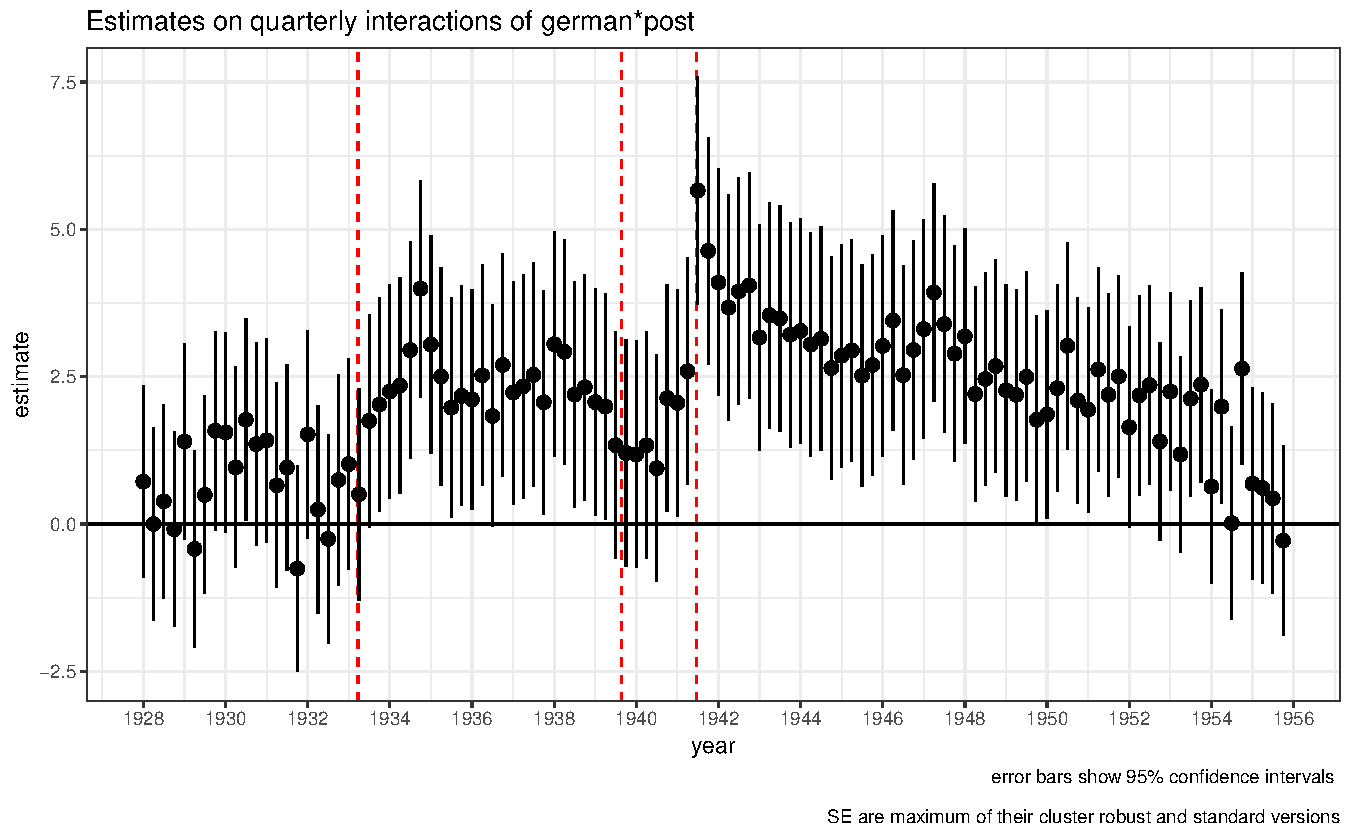
\includegraphics[width=\textwidth]{plots/effects/quarterly/pointrange.pdf}
\caption{Estimates of coefficients on $german \cdot post\_year$}
\label{fig_did_effets}
\end{figure}
%We perform several robustness checks to asses sensitivity of the results to different specifications. First, in our main model (column (1) of table \ref{dif_table}), we included all observations in years 1923 to 1958. But the relationship between Germany and Soviet Union were somewhat more complicated after the World War II. We thus re-estimate the model with only the data from 1923 to 1945. The results (in column (2)) change only little and does not alter our previous conclusions. Second, when we omit the ethnicity specific linear time trends in column (3), we see again that the coefficients are very similar to the original model. Finally, we estimate a specification with number of arrests as a dependent variable (without logarithmic transformation). We can see that this model (shown in column (4)) fits the data rather poorly with  $R^2$ only of 0.428 (compared to 0.890 in the logarithmic specification). 

\section{Synthetic Control Method}
However, the parrarel trends assumption can sometiemes be violated. These issues can be adressed by sythetic control method
\citep{abadie_synthetic_2010, abadie_economic_2003}. We closely follow \citet{abadie_synthetic_2010}.

Let $Y_{it}$ be log of number of arrests of individuals belonging to an ethnic group $i$ at time $t$ with $i = 1$ being German ethnicity.  We
denote $D_{1t}$ as the treatment dummy, i.e. variable that equals 1 if $i = 1$ and $T > \text{1933Q1}$ (Hitler's rise to power) and 0 otherwise. 
Let be $Y_{1t}^N$ be a counterfactual log of number of arrests of Germans in the absence of treatment. SCM assumes a model
\begin{equation}
    Y_{1t} = Y_{1t}^N + \alpha_{1t} \, D_{1t}
\end{equation}
Furthermore, we assume that $Y_{1t}^N$ is given by the following factor model:
\begin{equation}
   Y_{1t}^N = \delta_t + \boldsymbol{\theta}_t \boldsymbol{Z}_i +
   \boldsymbol{\lambda}_t \boldsymbol{\mu}_i + \epsilon_{it}
\end{equation}
where is $\delta_t$ an unknown common factor with constant factor
loadings across units, $\boldsymbol{Z}_i$ is a
$(1 \times r)$ vector of observed time-invariant covariates (unaffected by the treatment),  $\boldsymbol{\theta}_t$ is a $(1 \times r)$ vector of
unknown parameters, $\boldsymbol{\lambda}_t$ is a $(1 \times F)$ vector of unobserved time-varying factors, $\boldsymbol{\mu}_i$ is an $(F \times 1)$ vector of unknown factor loadings
and $\epsilon_{it}$ is the error term with zero mean. 

Notice that for constant  $\boldsymbol{\lambda}_t$ for all $t$ we get the traditional  difference-in-differences model. Unlike difference-in-differences,  the synthetic control method  allows for unit-specific time trends as long as they can be captured by the factor model. 

The synthetic control works by contracting a control group for which the average of its factor loadings $\boldsymbol{\mu}_i$ match the factor loadings of the treated unit  $\boldsymbol{\mu}_1$.

For pre-treatment

\subsection{Results}
Figure \ref{fig_sc_comp_plot} shows the outcome variable for synthetic group and actual.  
\begin{figure}[h]
\centering
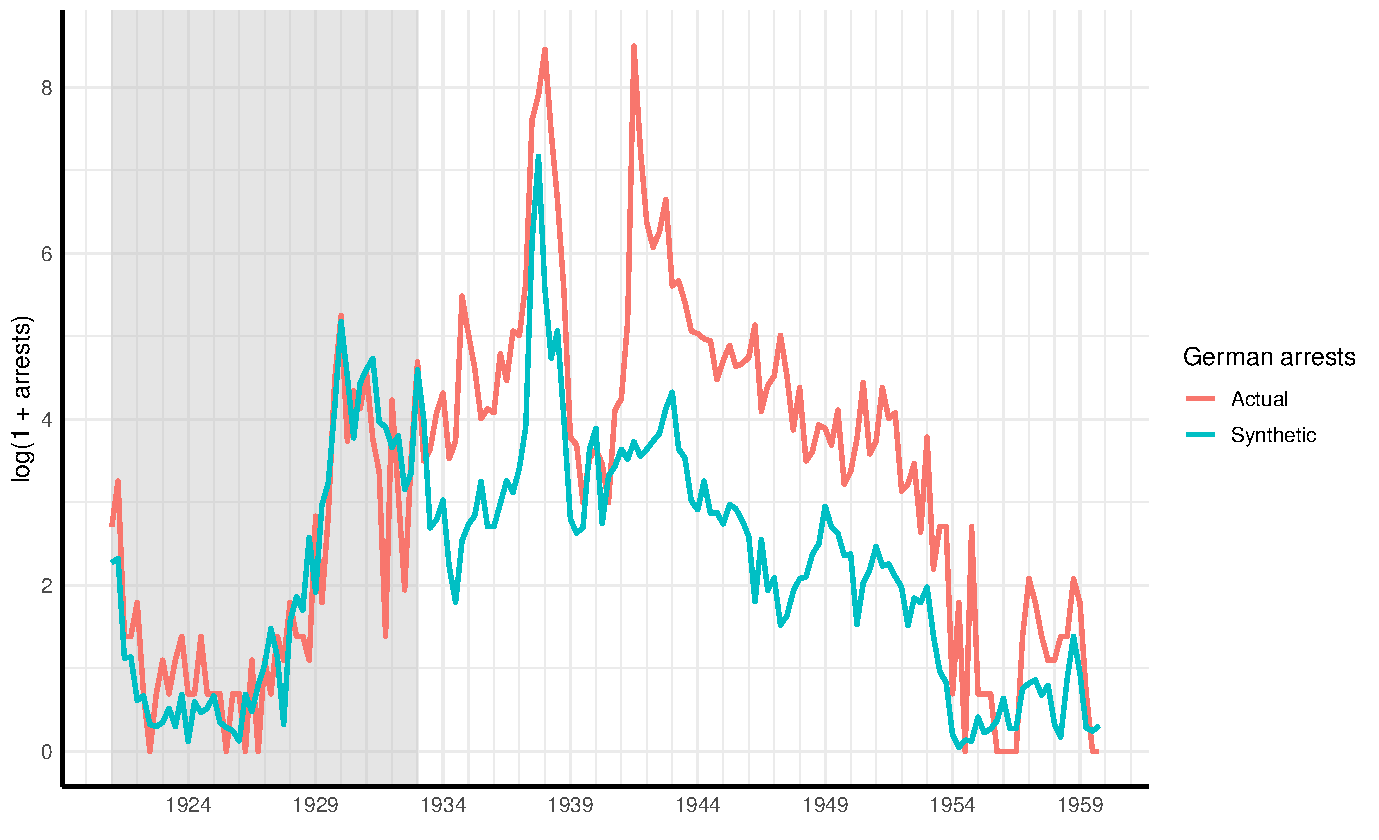
\includegraphics[width=\textwidth]{plots/synthetic_control/comparison_plot.pdf}
\caption{Comparison plot}
\label{fig_sc_comp_plot}
\end{figure}

Figure \ref{fig_sc_placebo_gaps} depicts the gaps in logarithm of quarterly arrests between the actual and synthetic groups for Germans together with gaps for all 17 other ethnic groups. 
\begin{figure}[h]
\centering
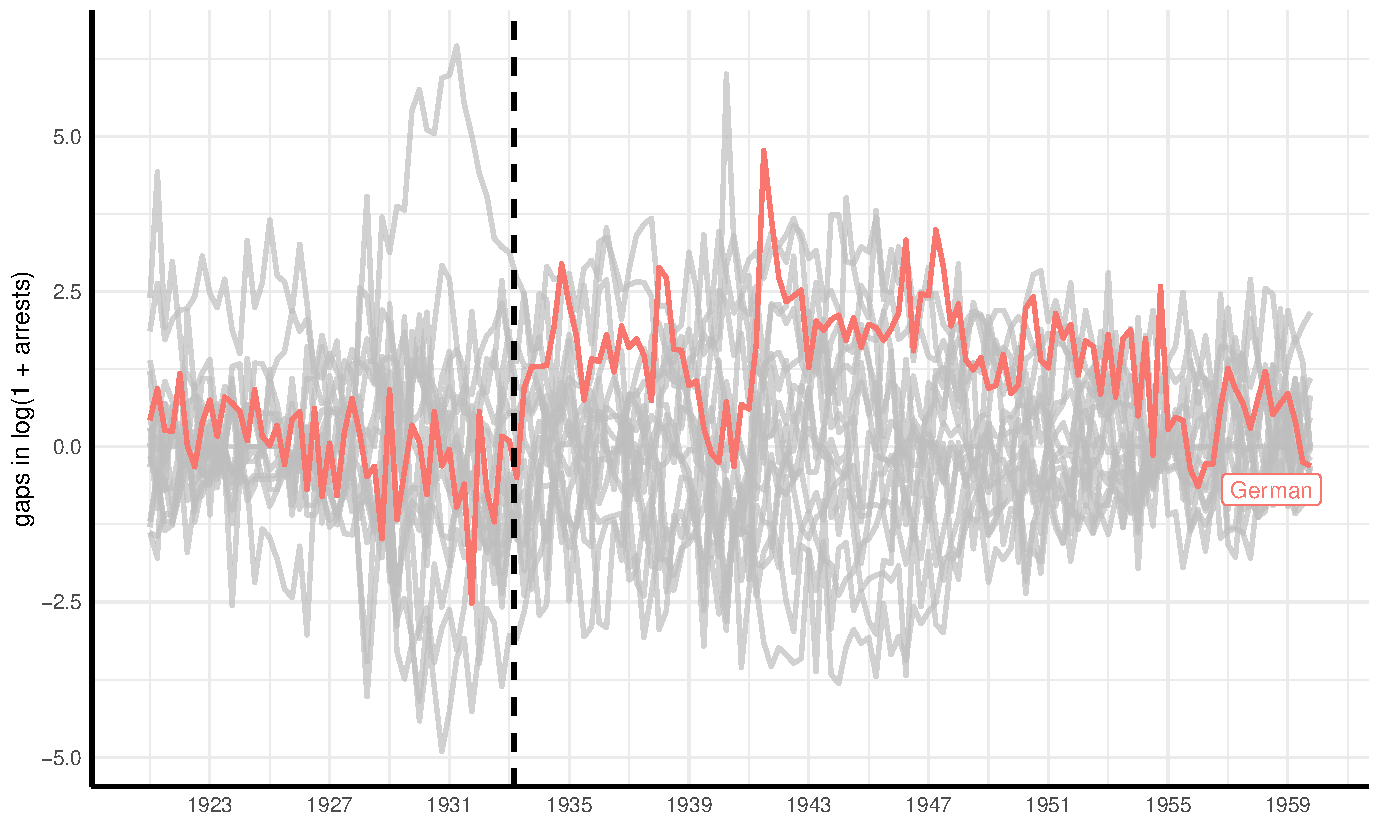
\includegraphics[width=\textwidth]{plots/synthetic_control/placebo_highlight_all.pdf}
\caption{Placebo gaps}
\label{fig_sc_placebo_gaps}
\end{figure}

This is shown in  the figure \ref{fig_sc_mspe_hist}
\begin{figure}[h]
\centering
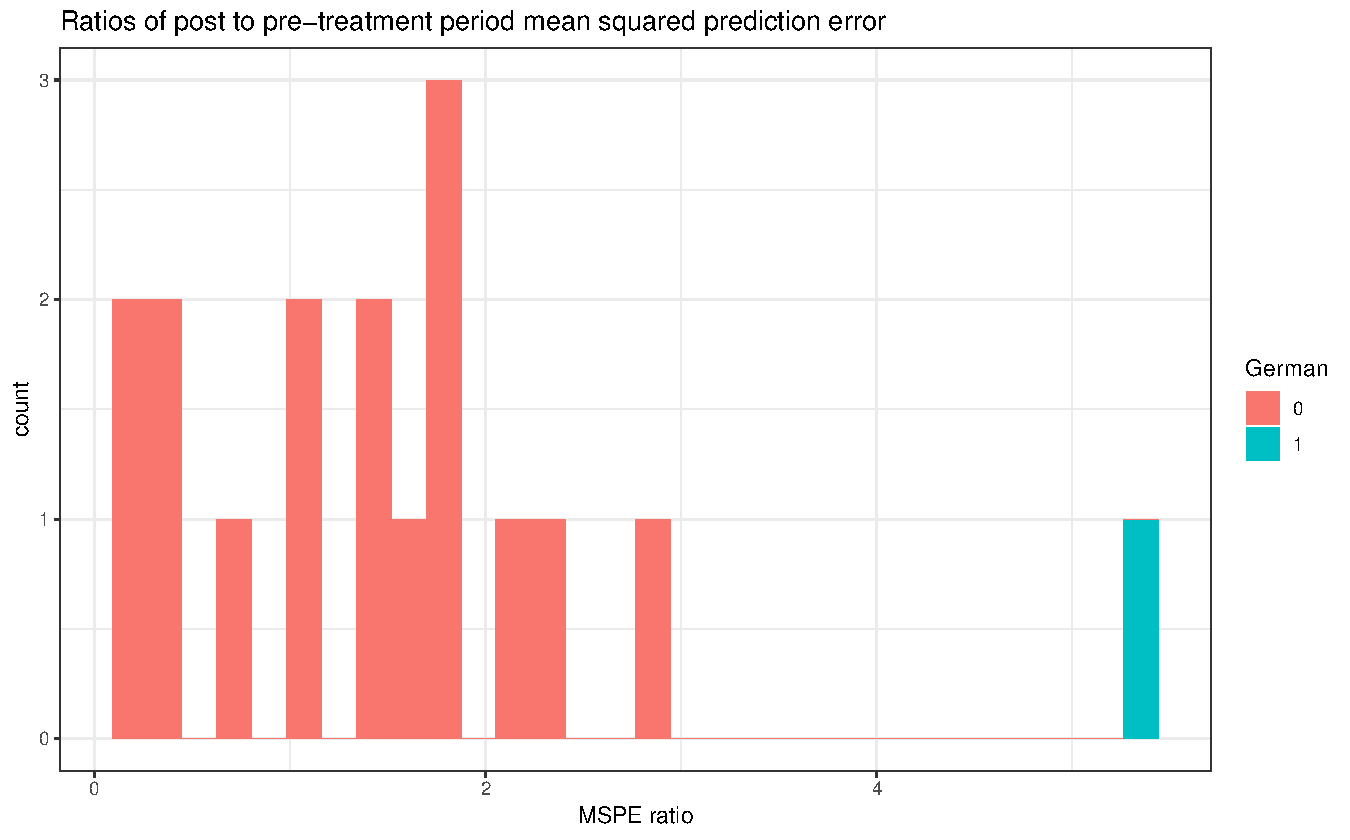
\includegraphics[width=\textwidth]{plots/synthetic_control/mspe_histogram.pdf}
\caption{Histogram of mean squared prediction error for all ethnicities}
\label{fig_sc_mspe_hist}
\end{figure}

Implemented in R software using the MSCM package \citep{becker_fast_2018}.
\subsection{Generalized Synthetic Control Method}
\citet{xu_generalized_2017}

\newpage
\section{Results} \label{sec:results}
\subsection{Difference-in-differences}
%In our main specification, we 
We first present results from our preferred specification \ref{eq:dynamic_did} with geopolitical controls and no ethnicity-specific time trends. 
The interaction of the specific year and German dummy variables is omitted only for 1921 which therefore serves as baseline for comparison with other years. 
All 38 ethnic groups in the dataset are included. 
We imputed missing ethnicity and date of arrest as described in the section \ref{sec:missing_data}.  Full matrix adjustment from equation \ref{eq:full_matrix_adj}) was applied to the ethnicity imputations. 
%We start by presenting results for the data with imputed ethnicity (adjusted with full matrix correction from equation \ref{eq:full_matrix_adj} and date of arrest since we consider them to be the most credible. However, we also consider how the results change if do not impute or apply different adjustment further in the paper. 

 The estimated coefficients  $\beta_k$ from the dynamic difference-in-differences model (\ref{eq:dynamic_did}) are plotted in the figure \ref{fig:did_effets}. Recall that our dependent variable  is $\log\left(1 + \text{arrests}_{it}\right)$ and therefore we can interpret the coefficients  $\beta_k$  as percentage change in arrests.
 We can draw several conclusions from the results. 
 First, the coefficients from 1933 to 1938 are all smaller than 1 and most of them are not significantly different from zero which implies that hostility between Germany and the Soviet Union in this period does not seem to impact the repressions of Germans contrary to the theoretical predictions. Second, the political arrests of Germans start to rise in 1939 which is surprising given that  Molotov-Ribbentrop pact guaranteeing neutrality Germany and the USSR was signed that year. The repressions then peak  in 1940 and 1941  at 4\%
  followed by sharp drop in years 1942-1944 to approximately 1.5\%. 
  %We have to be cautious when interpreting those 
  However,  we have to be careful when interpreting those coefficients. 
 Since the Soviet Union was at that period at war and initially lost large amounts of territory, it is plausible that the arrests of Germans  declined simply because there were fewer Germans on the territory controlled by the Soviets. 
 %(although there is some slight drop from 1942 to 1944). 
 In any case,  the impact of war on the repressions appear to be highly persistent as 
  the estimated effect stays high at around 2 to 3\% even after 1945.
Finally,  starting from 1955, the coefficients rapidly fall to zero. 
This period coincides with the partial relaxation of repressions and censorship following the death of Stalin in 1953 and the subsequent  rise of power of Khrushchev. 
This is reflected in our data where the number of arrested Germans in a given year after 1954 does not exceed 50 compared to hundreds of arrests in the preceding years.  

We can calculate based on these coefficients what number of repressions of Germans is attributable to the worse geopolitical situation according to our model. 
If we consider for example that for 1940 there are 21 205 arrests of Germans in our dataset and the coefficient for 1940 is 3.88 then the model implies that 822 of arrests were due to the geopolitical changes. 
If we repeat this for every year from 1933 to 1960, we get that total number of repressions attributable to these German-specific post-1933 changes is 4 148 out of 152 938. 
%To get information for the wh

%We can get better idea about magnitude of the effects by converting
%We can get better convert the percentage change into actual number
%To put these numbers into concrete terms, 

 %there tion is no decline in the arrests after 1945. 
 %The coefficients in the model imply that in the period of Molotov-Ribbentrop pact and war, the arrests of Germans were about 2\% higher than the arrest other ethnic groups. Surprisingly, the estimated effect in the post-war period is higher still at  3.6\%.
 \begin{figure}[h]
\centering
\caption{Estimates of $\beta_k$ from the Specification \ref{eq:dynamic_did}}
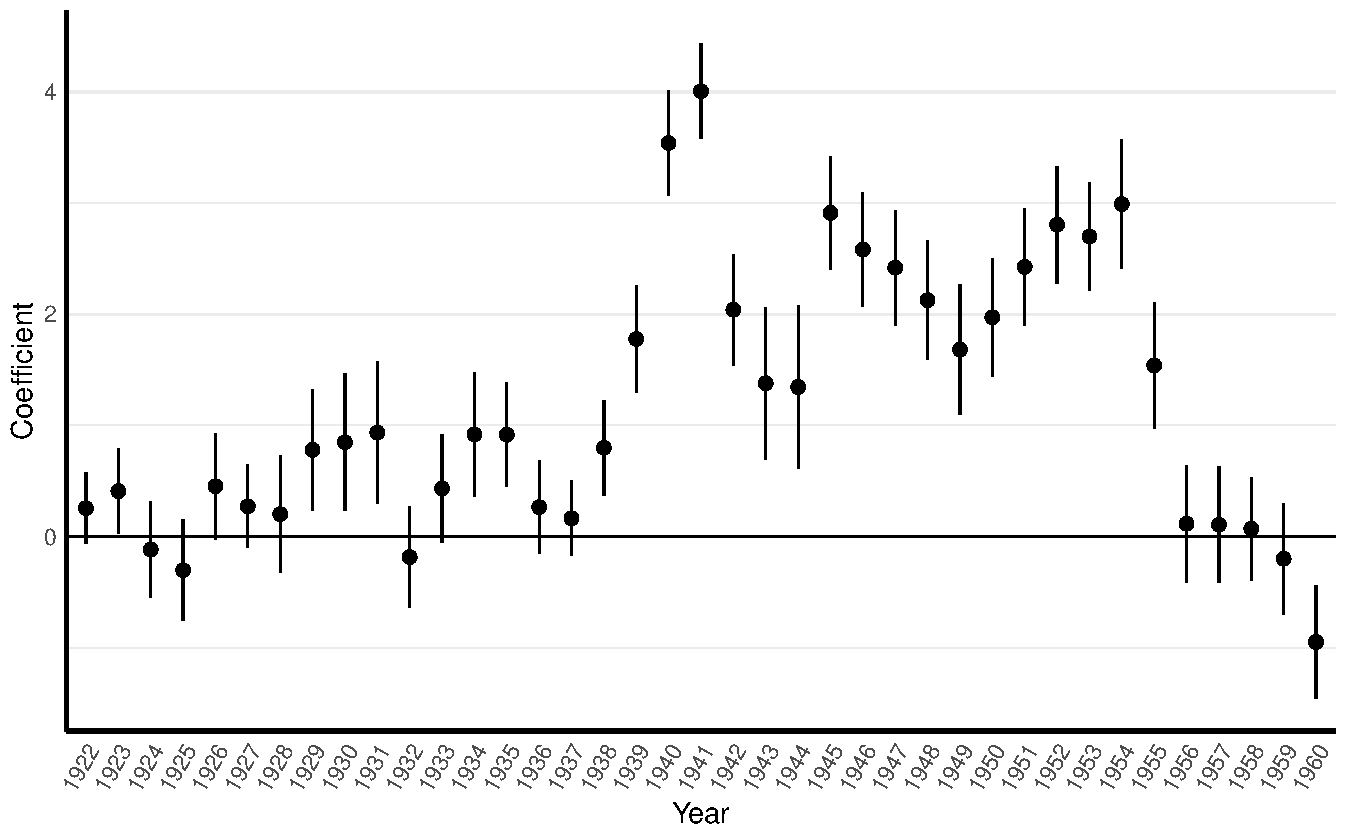
\includegraphics[width=\textwidth]{plots/final/fmla_pred_full_imp_date_no_trends_geopol_cr2.pdf}
\begin{minipage}{0.92\textwidth}
\footnotesize
\emph{Notes:} Ethnicity and date of arrest were imputed.  Full matrix adjustment was applied on ethnic group imputations. All 38 ethnic groups are included. 
There are no ethnicity-specific time trends. 
Standard errors are clustered on the level of ethnicity and are based on cluster robust estimator by \citet{pustejovsky_small-sample_2018}. Error bars show 95\% confidence intervals. 
\end{minipage}
\label{fig:did_effets}
\end{figure}

 
% The results from the time window specification (equation \ref{eq:simple_did}) shown in the figure \ref{fig:did_effets_time_window} tell the same story.  
 
% \begin{figure}[h]
%\centering
%\caption{Estimated Coefficients for Specified Time Windows from the Specification \ref{eq:simple_did}}
%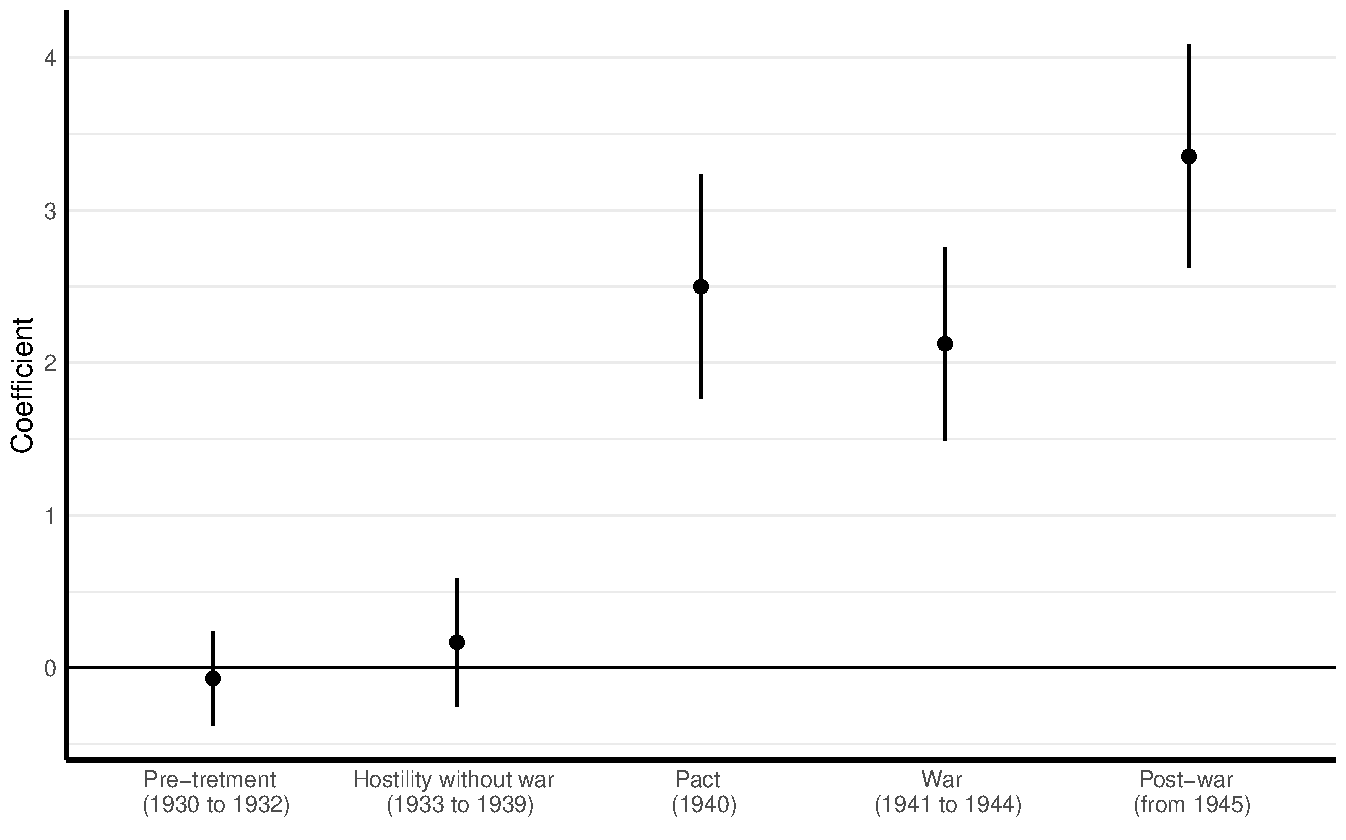
\includegraphics[width=\textwidth]{plots/effects/ethnicity_imputation/annual/time_window_pre_treatment_date_imp.pdf}
%\begin{minipage}{0.92\textwidth}
%\footnotesize
%\emph{Notes:} Ethnicity and date of arrest were imputed.  Full matrix adjustment was applied on ethnic group imputations. All 38 ethnic groups are included. Standard errors are based on cluster robust estimator by \citet{pustejovsky_small-sample_2018}. Error bars show 95\% confidence intervals. 
%\end{minipage}
%\label{fig:did_effets_time_window}
%\end{figure}
 
However, the pre-1933 coefficients in the figure \ref{fig:did_effets} give us some reason to doubt the
validity of our model. Even though they are small in size relative to the post-1939 coefficient, they are all  significantly different from 0 at 5\% level.
%and others are very close to being significant. 
This provide some evidence that the pre-treatment trends for German minority were not parallel with trends for other ethnic groups. We can thus suspect that the post-treatment trends were not parallel either which
would violate the basic identifying assumption of
difference-in-differences.
%The deviations from parallel trends in the pre-treatment period are relatively small possibly indicating that the bias might not be as large. 
We address this problem by applying the synthetic control method in the next section. 
%Nevertheless, the  deviations of pre-1933 from zero are small which coulf 
%Bearing in mind these potential problems, we proceed 
 
Another potential issue is that some ethnic groups changed their treatment status in this period in various complicated ways. 
We tried to control for this by including a set of dummy variables  that capture the most important changes in geopolitical relations (more on their definition in appendix). 
However, these dummy variables might miss  more subtle changes in relations with the USSR. As a robustness check, we therefore exclude every ethnicity which constituted a core group in some independent state in the interwar period from the dataset (except for Germans, of course) and reestimate the model. This criterion removes 10 ethnic groups from the dataset. The full list of them is provided in the table \ref{tab:sc_predictors}. The results of the dynamic difference-in-differences are plotted in the figure \ref{fig:did_effets_no_ind_countries} in the appendix. The estimated coefficients change  very little compared to the results with all ethnic groups included, only confidence intervals appear slightly wider since we have fewer observations. Therefore our previous results are maintained. 

%For example, Poland was invaded by the USSR and Germany but it took  only about month until the Polish forces were defeated. The Baltic states were annexed and incorporated into the Soviet Union in June 1940 only to be invaded by Germany year later. 
%It is difficult to decide what treatment status should we assign in these cases. 
%Moreover, given the scale and complexity of World War 2, the USSR experienced  some kind of change in geopolitical relations with almost every country in its neighborhood.  

%To address this issue, we exclude every ethnicity which constituted a core group in some independent state in the interwar period from the dataset (except for Germans, of course) and reestimate the model. This criterion removes 10 ethnic groups from the dataset. The full list of them is provided in the table \ref{tab:sc_predictors}. The results of the dynamic difference-in-differences are plotted in the figure \ref{fig:did_effets_no_ind_countries} in the appendix. The estimated coefficients change  very little compared to the results with all ethnic groups included, only confidence intervals appear slightly wider since we have fewer observations. Therefore our previous results are maintained. 

In the section \ref{subsec:robust_checks}, we perform several additional robustness checks to further asses the sensitivity of our findings. In particular, we refit the models for different ethnicity-specific time-trends and imputation adjustments. 

%Bearing in mind these potential problems, we continue by considering different sets of control groups to better understand what drives the results. 
 
 %The coefficients between the years 1933 and 1939 (when the relations between Germany and Soviet Union were hostile) mostly range  between 1 and 3 and all except one are statistically significant at 5\% level. The rise of Nazism thus based on these estimated increased the arrests of Germans by the NKVD in the USSR by about 2\%.  

%However, the pre-1933 coefficients give us some reason to doubt the
%validity of our model. Three of them are significantly different from 0 at 5\% level and others are very close to being significant. 
%This provide some evidence that the pre-treatment trends for German minority were not parallel with trends for other minorities. We can thus suspect that the post-treatment trends were not parallel either which would violate the basic identifying assumption of difference-in-differences. To address this concern, we apply the synthetic control method which can be valid even in the absence of  parallel trends. 
%We can see that all coefficients for years 1930 to 1932 are statistically insignificant which means that the pre-treatment trends in arrests of German minority were likely parallel to the pre-treatment trends of other minorities which gives us greater  confidence in the validity of our identification strategy. 

%The coefficients on all other years are insignificant as well. Only for 1934 (one year lag) is the estimate  significant at 10\% level ($p$-value of 0.08). Since this not reaches even the traditional 5\% significance threshold we are inclined to not reject the null hypothesis or at least to conclude that evidence in favor of the alternative hypothesis (more repressions of Germans due to rise of Hitler) is quite weak.  Furthermore, as we show below the alternative specifications do not increase the significance of the coefficients.






%We perform several robustness checks to asses sensitivity of the results to different specifications. First, in our main model (column (1) of table \ref{dif_table}), we included all observations in years 1923 to 1958. But the relationship between Germany and Soviet Union were somewhat more complicated after the World War II. We thus re-estimate the model with only the data from 1923 to 1945. The results (in column (2)) change only little and does not alter our previous conclusions. Second, when we omit the ethnicity specific linear time trends in column (3), we see again that the coefficients are very similar to the original model. Finally, we estimate a specification with number of arrests as a dependent variable (without logarithmic transformation). We can see that this model (shown in column (4)) fits the data rather poorly with  $R^2$ only of 0.428 (compared to 0.890 in the logarithmic specification). 

%We perform several robustness checks to asses sensitivity of the results to different specifications. First, in our main model (column (1) of table \ref{dif_table}), we included all observations in years 1923 to 1958. But the relationship between Germany and Soviet Union were somewhat more complicated after the World War II. We thus re-estimate the model with only the data from 1923 to 1945. The results (in column (2)) change only little and does not alter our previous conclusions. Second, when we omit the ethnicity specific linear time trends in column (3), we see again that the coefficients are very similar to the original model. Finally, we estimate a specification with number of arrests as a dependent variable (without logarithmic transformation). We can see that this model (shown in column (4)) fits the data rather poorly with  $R^2$ only of 0.428 (compared to 0.890 in the logarithmic specification). 


\subsection{Synthetic Control Method}
We implemented the synthetic control method in R  using the MSCMT package \citep{becker_fast_2018}.
Our outcome variable is again $\log\left(1 + \text{arrests}\right)$.
As in the difference-in-difference, we include all 38 ethnic groups and we impute missing date of arrest and ethnicity (which we adjust using the full-matrix correction).
In our baseline model, the  outcomes for all pre-treatment years (1921-1932)  were included  as predictors. 
This approach has been widely used in the literature \citep{billmeier_assessing_2013, cavallo_catastrophic_2013, bohn_did_2014} and in contrast to other methods (such as using only mean of pre-treatment outcomes) it  has the advantage  of reducing opportunities of specification search  \citep{ferman_cherry_2018}. 
We also include three time-invariant covariates that might potentially be predictive of post-1933 repressions: total population of the ethnic group in the USSR, its urbanization rate (both taken from the 1926 Soviet census), and linguistic similarity to Russian. 
However, including all pre-treatment outcomes as predictors  renders  other  covariates unimportant in the optimization procedure \citep{kaul_synthetic_2018}. On the other hand, \citet{botosaru_role_2019} argue that if there is a long set of pre-treatment outcomes (which is our case) then a perfect balance on covariates should not be required.
Since there is no clear consensus in the literature, we apply both methods and show the synthetic control method with mean of the pre-treatment outcome as predictor in section \ref{subsec:robust_checks} as a robustness check in addition to our baseline specification with  all pre-treatment outcomes as predictors that we present below. 

% Taken together, our results show that, while there may be advantages in balancing on covariates to construct the SC estimator, a perfect balance on covariates should not be required for the SC method, as long as there is a perfect balance on a long set of pre-treatment outcomes. O


The calculated optimal weights $W$ of ethnic groups in the synthetic German minority are provided in the table \ref{tab:sc_weights} (ethnic groups with zero weight are not shown). The highest contribution in the synthetic German minority have Russians, Greeks and Finns with weights 0.36, 0.28, and 0.17 respectively.  Lithuanians, the Khakas, Yakuts, and Bulgarians  are also represented in the synthetic control although only with  weights smaller than 0.08. 
\begin{table}[t]

\caption{\label{tab:sc_weights}Synthetic German minority weights}
\centering
\begin{tabular}{lr}
\toprule
Ethnic group & \$W\$-Weight\\
\midrule
Greek & 0.32\\
Kabardian & 0.09\\
Chuvash & 0.08\\
Moldovan & 0.07\\
Belorussian & 0.06\\
Polish & 0.06\\
Finnish & 0.06\\
Altai & 0.04\\
Armenian & 0.04\\
Georgian & 0.03\\
Ossetian & 0.02\\
Chechen & 0.02\\
Kazakh & 0.02\\
Bashkir & 0.02\\
Jewish & 0.02\\
Ukrainian & 0.01\\
Bulgarian & 0.01\\
Latvian & 0.01\\
Chinese & 0.00\\
\bottomrule
\end{tabular}
\end{table}

%The balance of covaria
%\begin{table}[!h]

\caption{\label{tab:sc_predictor_means}Pre-treatment Predictor Means}
\centering
\begin{threeparttable}
\begin{tabular}{lrrr}
\toprule
\multicolumn{1}{c}{ } & \multicolumn{2}{c}{German minority} \\
\cmidrule(l{2pt}r{2pt}){2-3}
Variable & Actual & Synthetic & Mean of all 38 ethnicities\\
\midrule
Log(1 + arrests) & 5.59 & 5.59 & 3.65\\
Total population & 1 238 549.00 & 28 292 179.83 & 3 681 250.42\\
Urbanization rate & 14.92 & 20.96 & 17.84\\
Ling. similarity to Russian & 1.00 & 2.29 & 0.76\\
\bottomrule
\end{tabular}
\begin{tablenotes}
\item \textit{Note: } 
\item Log(1 + arrests) is averaged over the pre-treatment period (1921-1932). All other predictor are time-invariant. Total population and urbanization rate are taken from 1926 Soviet census.
\end{tablenotes}
\end{threeparttable}
\end{table}


Figure \ref{fig:sc_comp_plot} shows the  arrests of the German minority and its synthetic control.
The synthetic control fits the actual pre-treatment values reasonably well. 
In the post-treatment period, both time series follow similar general trends (rise in 1937-1938 and decline after 1945). 
However up until 1955, the actual arrests of Germans are consistently higher than the predictions of  synthetic control. %We can get more detailed picture in 
We can infer the estimated effect size in the post-1933 period  from 
the figure  \ref{fig:sc_placebo_gaps_all} which shows the difference between the actual arrest and their synthetic counterparts for each year (on $\log(1 + x)$ scale). 

 \begin{figure}[h]
\centering
\caption{Comparison plot}
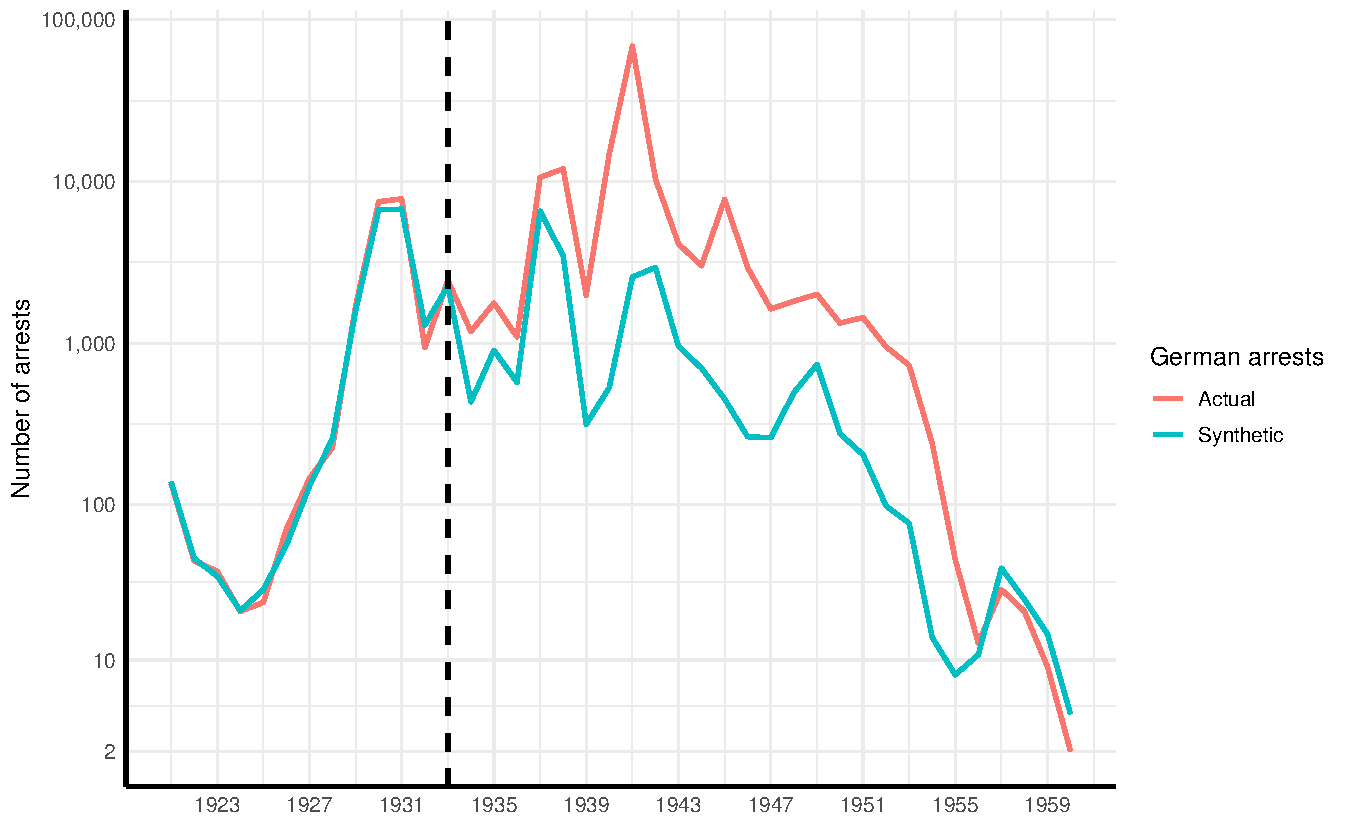
\includegraphics[width=\textwidth]{plots/synthetic_control/ethnicity_imputation/annual/comparison_plot_scaled.pdf}
\begin{minipage}{0.92\textwidth}
%\includegraphics[width=\linewidth]{Gaus.pdf}
%\rule{\linewidth}{10em}
\footnotesize
\emph{Notes:} The values on y-axis are shown on $\log\left(1 + y\right)$ scale.  Ethnicity and date of arrest were imputed.  Full matrix adjustment was applied on ethnic group imputations. All 38 ethnic groups are included. 
\end{minipage}
\label{fig:sc_comp_plot}
\end{figure}


From 1933 to 1939, this gap is close to 1. For the period from 1941 to 1955, the estimated effect is higher but also more volatile oscillating between 1 and 3 corresponding to 1 to 3\% increase in arrests of Germans in that period.  After 1955, the gap shrinks to zero. 
The results are similar to difference-in-differences in the overall trends. Nevertheless, the estimated effects by the  the synthetic control  are slightly smaller than the their difference-in-differences equivalents.  

%As we metioned in the section
We estimate the significance of our results with placebo tests by applying the same procedure to every ethnic group in the dataset. The differences between the actual values and the respective synthetic control for every placebo ethnicity are plotted in grey in the figure \ref{fig:sc_placebo_gaps_all}. Even in comparison with the placebo tests, 
the estimated effect for German ethnicity  still appears relatively large for the period from 1939 to 1955 although for years 1933-1938 the effect for Germans seems within the standard range of the placebo gaps.

The figure \ref{fig:sc_placebo_gaps_all} also shows that for some ethnic groups the pre-treatment gaps are large.
 For example, the gap for Russians stays above 2.5 for the whole pre-1933 period. 
 This indicates that synthetic control of these ethnic groups does not capture the actual pre-treatment trends well. 
 %In other words, no linear combination of ethnic group cannot 
 As we explained in the subsection \ref{subsec:sc_methodology}, the placebo synthetic controls  with with substantially  worse pre-treatment then the treated unit should not be 
used in estimating significance of the treatment effect. 
%are not very helpful for
%for estimating rareness of an effect for a treated unit with a good pre-treatment fit. 
We thus  exclude the placebo ethnicities whose pre-treatment mean squared prediction error (MSPE) is 20 times higher than the same measure for German minority. Even though this is relatively lenient cutoff, it removes 11 ethnic groups that does not meet the criterion. 
The resulting plot is shown in the figure \ref{fig:sc_placebo_gaps_all_20_times}. The post-1933 gaps in German arrests now stand out more clearly and even the gap for the years 1933-1938 now appears relatively significant.  
%They thus recommend excluding excluding placebo groups with substantially higher pre-treatment mean squared prediction error  (MSPE)

%Following \citet{abadie_synthetic_2010}  we therefore exclude ethnic groups whose pre-treatment MSPE is 5 times higher then the same measure for German minority. This removes 4 ethnic groups with the worst pre-treatment fit. The resulting plot is shown in the figure \ref{fig:sc_placebo_gaps_all_20_times}. The post-1933 gaps in German arrests now stand out more clearly. 


%The trends start to diverge in the second quarter of 1933 with the actual arrests of Germans holding steady but decreasing for synthetic control. 
%The gap between the trends for the actual German minority and its synthetic control (shown in figure \ref{fig:sc_placebo_gaps_all}) keeps within the range of 1.25 to 2.5 for most of the post-1933 period. This implies that the rise of Hitler led to about  2\% increase in the arrests of Germans by the NKVD  in the period from 1933 to 1939. This is very similar to the estimates obtained using difference-in-differences. 
%The figure shows increase between 1937 and 1939 (the period of the Great Terror).  




%\subsubsection{Inference}
%The estimated  gaps between the synthetic control and the actual data for every ethnic group is shown in figure \ref{fig:sc_placebo_gaps}. 

%are not very helpful for
%for estimating rareness of large  post-treatment gap for a treatment with a good pre-treatment fit. They thus recommend excluding excluding placebo groups with substantially higher pre-treatment mean squared prediction error  (MSPE)
%(the average of squared differences between the value of the outcome for synthetic and actual) 
%relatively to the treated group. 
%In our case the pre-treatment MSPE of the German minority is fairly small (0.52). 
%If we exclude minorities with the pre-treatment MSPE
%If we choose the cutoff for exclusion as the MSPE 

%Morever, the pre-treatment MSPE is quite small (0.52) which means that the synthetic German minority captures the actual pre-treatment trends relatively well. However, the pre-treatment MSPE of a few minorities is much larger indicating that no combination of donor ethnic groups fits well their time series. As \citet{abadie_synthetic_2010} note,  if there is poor fit of the synthetic control to the actual trends in the pre-treatment period then its post-treatment gap does not provide good comparison to the well fit ethnic groups. 
%large post-treatment gap would not indicate the presence of an effect but  
%Following \citet{abadie_synthetic_2010}  we therefore exclude ethnic groups whose pre-treatment MSPE is 5 times higher then the same measure for German minority. This removes 4 ethnic groups with the worst pre-treatment fit. The resulting plot is shown in the figure \ref{fig:sc_placebo_gaps_all_5_times}. The post-1933 gaps in German arrests now stand out more clearly. 

\begin{figure}[hbtp] 
\caption{Gaps between synthetic control and actual values for placebo tests}
\begin{subfigure}{\textwidth}
\caption{All ethnic groups}
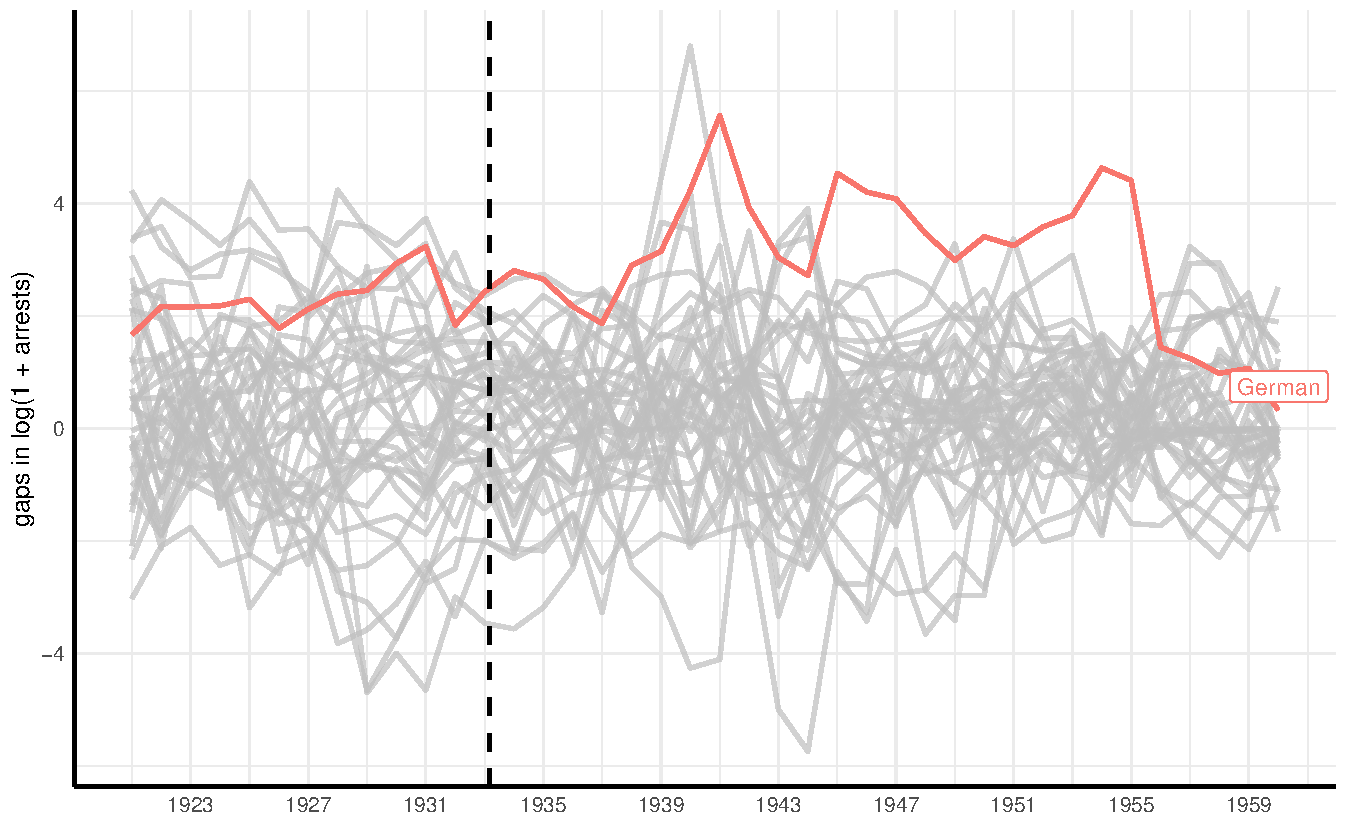
\includegraphics[width=0.9\linewidth]{plots/synthetic_control/ethnicity_imputation/annual/placebo_highlight_all_imp_date.pdf}
\label{fig:sc_placebo_gaps_all}
\end{subfigure}
\begin{subfigure}{\textwidth}
\caption{Ethnicities with pre-treatment MSPE higher than 20 times the MSPE of Germans excluded}
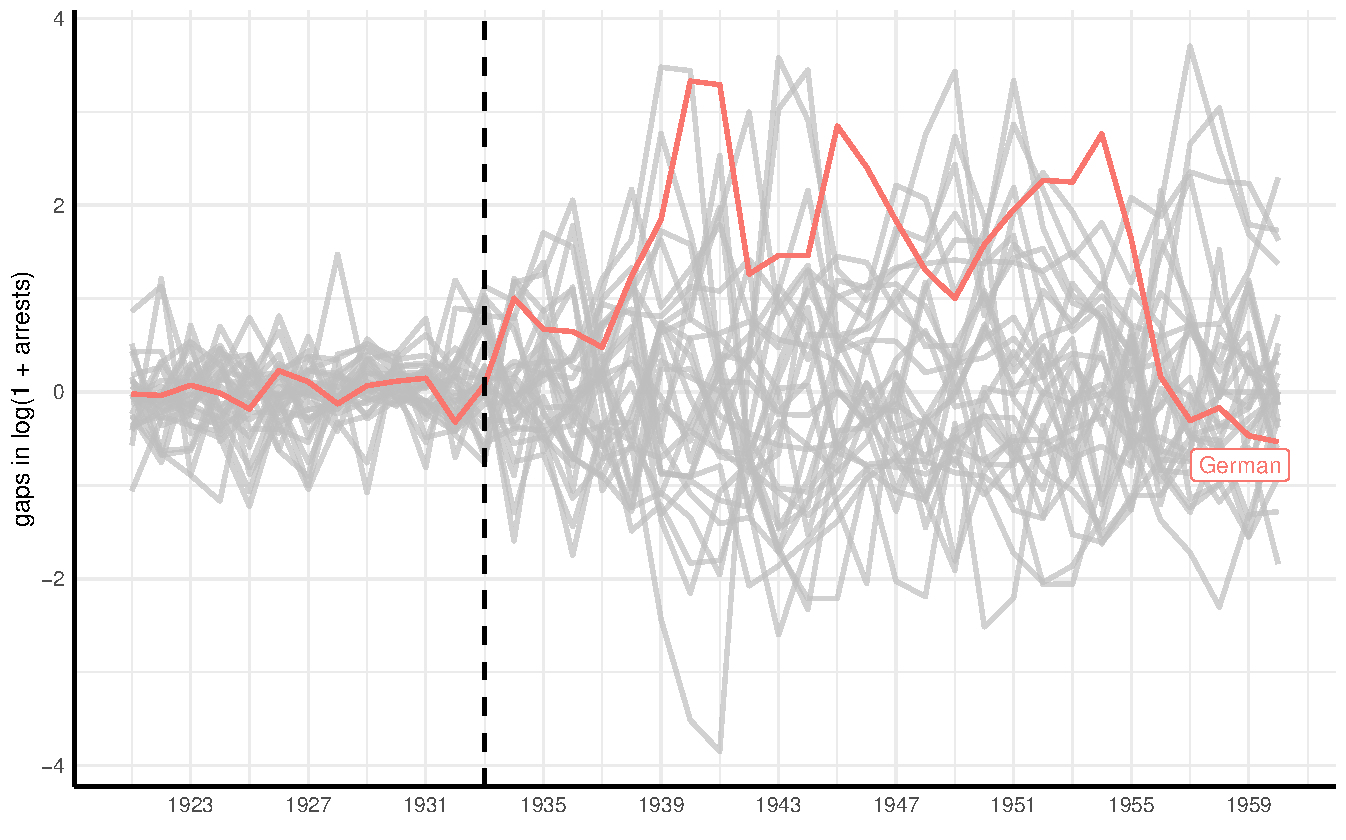
\includegraphics[width=0.9\linewidth]{plots/synthetic_control/ethnicity_imputation/annual/placebo_highlight_mspe_20lower_imp_date.pdf}
%Ethnic groups with pre-treatment MSPE higher than 5 times the MSPE of Germany excluded
\label{fig:sc_placebo_gaps_all_20_times}
\end{subfigure}
\label{fig:sc_placebo_gaps}
\end{figure}

Nevertheless, our preferred approach for assessing uncertainty in results that avoids  choice of any arbitrary level of the pre-treatment MSPE cutoff for the exclusion of poorly fit  placebos
is to compare the ratios of  post/pre-treatment MSPE. 
The values of these ratios for all ethnic groups are displayed in the figure \ref{fig:sc_mspe_ratios_all} for the whole post-treatment period. The MSPE ratio for the German minority is by far the highest. The probability of German minority having the highest ratio of all under the null hypothesis of zero treatment effect is 1/38 ($\approx 0.026$). 
In the figure \ref{fig:sc_mspe_ratios_until_1939}, we also provided the MSPE ratios  with the post-treatment MSPE calculated only for the years 
1933-1939  to estimate the significance just for this period. Although the gap between  MSPE ratio for German minority and other ethnic groups shrunk somewhat, the German MSPE ratios stays the highest and therefore we again get the  $p$-value of 1/38. 
These results contradict our inferences from difference-in-differences  where we could not reject the hypothesis of zero treatment effect for the period from 1933 to 1939. 


\begin{figure}[hbtp] 
\caption{Ratios of post-treatment MSPE to pre-treatment MSPE}
\begin{subfigure}{\textwidth}
\caption{The whole post-treatment period in the numerator (1933-1960)}
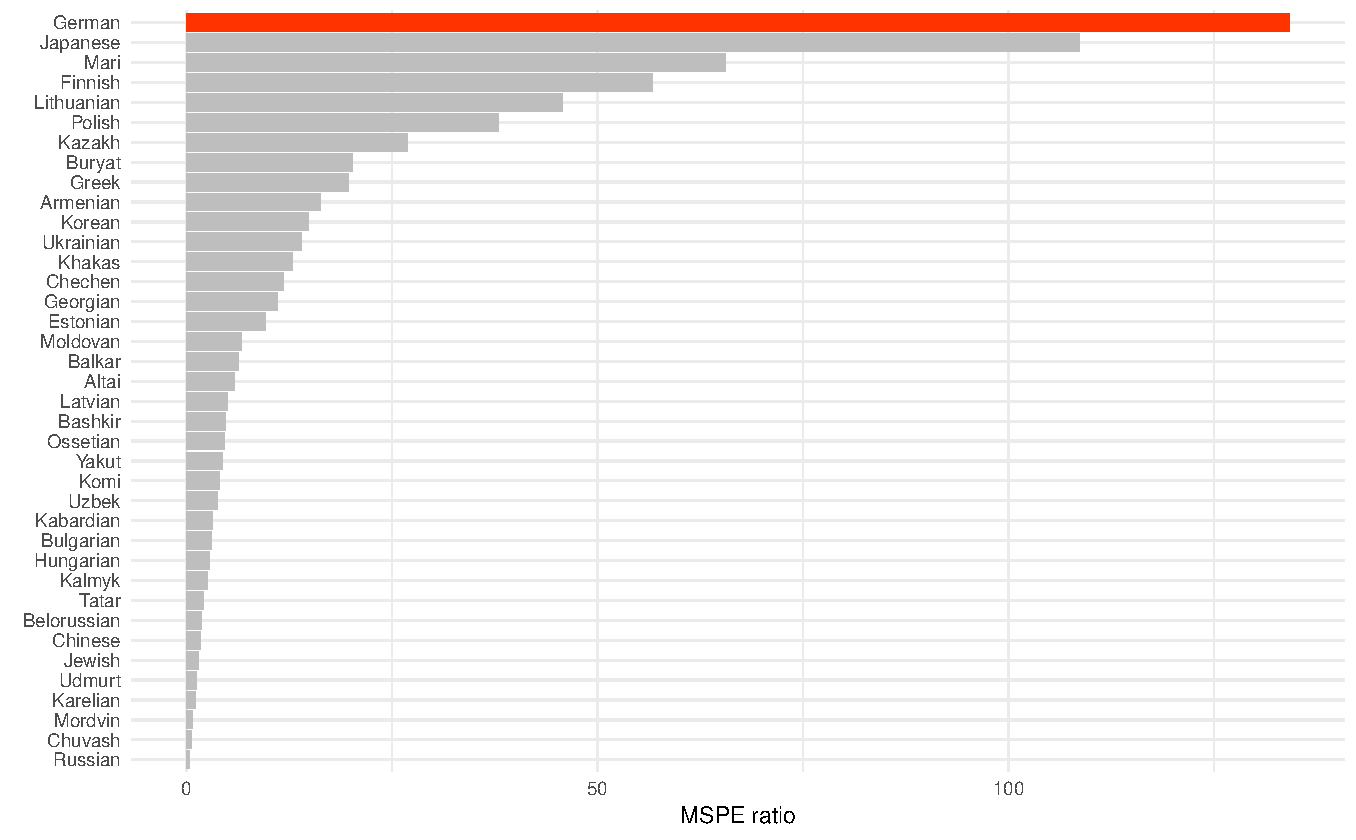
\includegraphics[width=\linewidth]{plots/synthetic_control/ethnicity_imputation/annual/mspe_ratios_imp_date.pdf}
\label{fig:sc_mspe_ratios_all}
\end{subfigure}
\begin{subfigure}{\textwidth}
\caption{Only the period from 1933 to 1939 in the numerator}
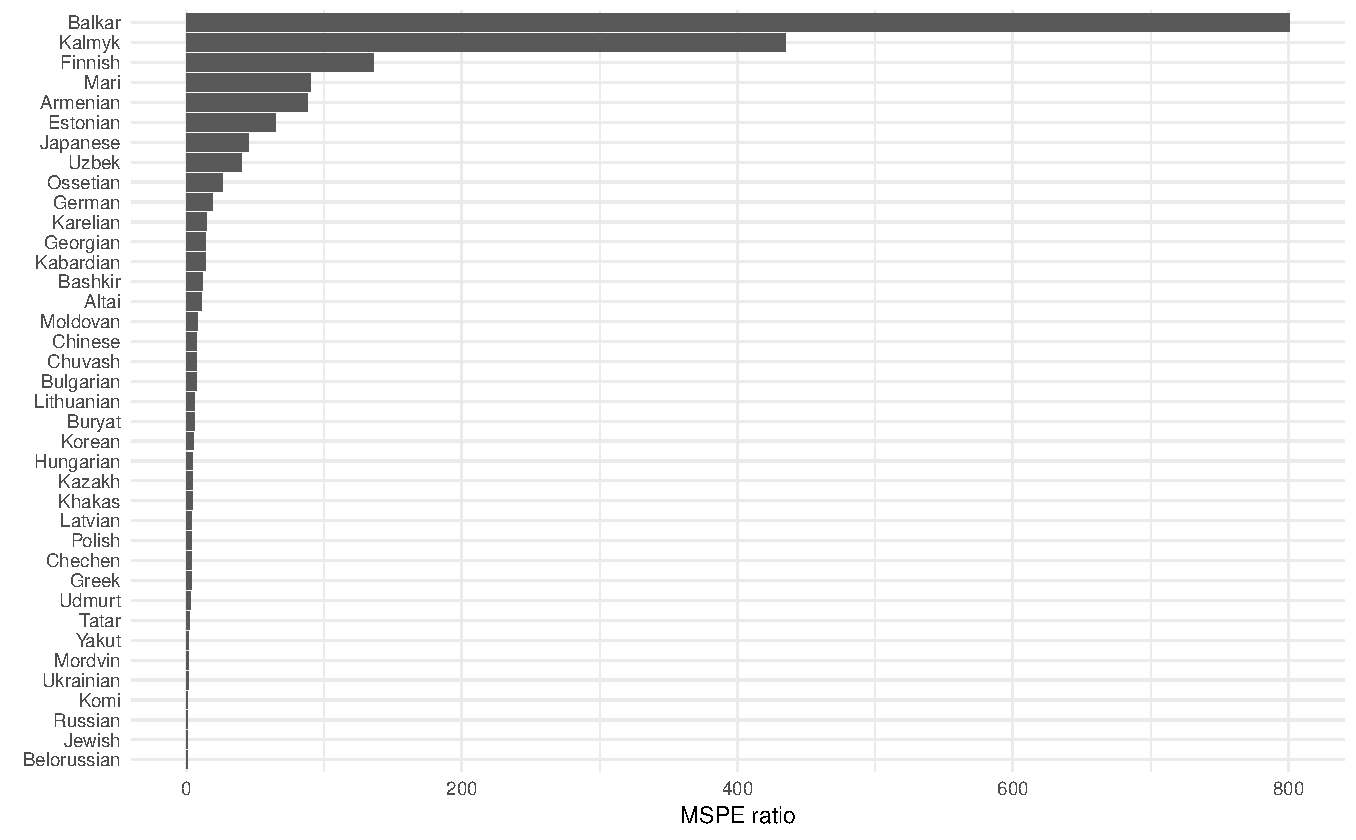
\includegraphics[width=\linewidth]{plots/synthetic_control/ethnicity_imputation/annual/mspe_ratios_imp_date_until_1939.pdf}
%Ethnic groups with pre-treatment MSPE higher than 5 times the MSPE of Germany excluded
\label{fig:sc_mspe_ratios_until_1939}
\end{subfigure}
\label{fig:sc_mspe_ratios}
\end{figure}


%This is shown in  the figure \ref{fig_sc_mspe_hist}


\section{Robustness Checks} \label{subsec:robust_checks}
\subsection{Difference-in-differences}

Our results have shown rise of arrests of Germans during and after the war. 
However, the question is if these people were arrested for aiding the invading German army or only based on their ethnicity. 
%We  try to answer this by restricting  our analysis to only rehabilitated individuals. 
Since the  Russia’s 1991 Law  \enquote{On Rehabilitation of Victims of Political Repression} specified  that individuals who joined the German army\footnote{Subsequent amendments expanded the restriction to anyone who aided the German army. }  were not eligible for rehabilitation, we can filter out the cases of direct 
cooperation by restricting  our analysis to only rehabilitated victims \citep{frierson_russias_2014}. 
In the Memorial database, there  are 1 257 796 individuals  classified as  rehabilitated (for rest of the data we either do not have the information on rehabilitation or they were not eligible for rehabilitation).  We thus re-estimate our baseline specification using only those observations. The results are plotted in the figure \ref{fig:did_effects_rehabs}. We see that the coefficients after 1933 change only little. Nonetheless, the pre-treatment estimates deviate from zero more. 
%this is a consequence of h

Second, we consider if the inclusion of ethnicity-specific time trends affects the results.
%As we discussed in the section \ref{subsec:methodology_did}, ethnicity-specific time trends can test if the t
%As we explained in the methodology section, 
% the ethnicity-specific time trends allows us. 
The estimates regressions with quadratic , linear, and no time (default) trends are  plotted in the figure \ref{fig:did_robustness_time_trends} in the appendix. The coefficients for the model with no ethnicity-specific time trends are somewhat lower for the baseline model and the estimates for linear time trends are lower still. Nonetheless, the main general pattern is preserved in all specifications.

Third, we test the sensitivity of results to different adjustments of ethnicity imputation. 
As we explain in the subsection \ref{subsubsec:pred_adj}, the adjustments were applied in order to correct for the unbalanced accuracy in prediction of our Naive Bayes classifier across ethnic groups. The results from fitting our default specification to data with different adjustments are shown in the figure \ref{fig:did_robustness_pred_adj}.
We see that the estimates for the full matrix (used by default) and the parsimonious adjustment are virtually the same. When no adjustment is applied, the coefficients even get slightly larger. 

%Forth, we omit different sets of interactions of the  year and German dummy variables to change the baseline against which the estimated coefficients are compared. In all previous specifications the only omitted year was 1921. In figure \ref{}

Finally, we also consider different type of standard errors. 
So far we have only used the cluster-robust estimator by \citet{pustejovsky_small-sample_2018} for the reasons explained in the subsection \ref{subsec:methodology_did}. 
This estimator uses biased reduced linearlizations
Alternative method for estimation of standard errors  in case of serial correlation and small number of clusters is to use number of clusters as a degrees of freedom. 
%As we mentioned in the subsection \ref{subsec:methodology_did}, our default 
\subsection{Synthetic Control Method}
 We construct a synthetic control  using mean of the outcome in the pre-1933 period instead of including outcome for every year as we did in our baseline model. This increases the importance of the time-invariant covariates (population, urbanization rate, and linguistic similarity) that are also included as predictors.
\begin{table}[!h]

\caption{\label{tab:sc_predictor_means_robustness}Pre-treatment Predictor Means}
\centering
\begin{threeparttable}
\fontsize{10}{12}\selectfont
\begin{tabular}{lrrrr}
\toprule
\multicolumn{1}{c}{ } & \multicolumn{2}{c}{German minority} \\
\cmidrule(l{2pt}r{2pt}){2-3}
Variable & Actual & Synthetic & Mean of all ethnicities & $V$ weights\\
\midrule
Log(1 + arrests) & 5.59 & 5.48 & 3.649 & 0.15\\
Total population & 1 238 549.00 & 1 747 879.23 & 3 681 250.421 & 0.84\\
Urbanization rate & 14.92 & 21.56 & 17.844 & 0.00\\
Ling. similarity to Russian & 1.00 & 1.16 & 0.763 & 0.00\\
\bottomrule
\end{tabular}
\begin{tablenotes}
\item \textit{Note: } 
\item Log(1 + arrests) is averaged over the pre-treatment period (1921-1932). All other predictor are time-invariant. Total population and urbanization rate are taken from 1926 Soviet census.
\end{tablenotes}
\end{threeparttable}
\end{table}

Recall that the predictors weights $V$ are chosen to minimize pre-treatment MSPE. We can thus infer from the calculated  weights $V$ (provided in the table \ref{tab:sc_predictor_means_robustness})  that neither urbanization rate nor linguistic similarity to Russian are good predictors of pre-1933 repressions. 
%Total population seems to be the most powerful predictor.
Therefore the $W$-weights of ethnic groups in the synthetic control are chosen to mainly match the German minority on population and the mean of $\log\left(1 + \text{arrests}\right)$. 
 The calculated $W$-weights  are shown in the table \ref{tab:sc_weights_robustness}. We see that Tatar and Polish minorities are now contributing with the largest share to the synthetic control. 

\begin{table}[t]

\caption{\label{tab:sc_weights}Synthetic German minority weights}
\centering
\begin{tabular}{lr}
\toprule
Ethnic group & $W$-Weight\\
\midrule
Tatar & 0.49\\
Polish & 0.39\\
Korean & 0.12\\
\bottomrule
\end{tabular}
\end{table}

When we compare the gaps between synthetic control and actual value (figure \ref{fig:sc_placebo_gaps_robustness}) with our baseline model, we notice three main differences. First, pre-treatment fit for Germany is substantially worse which is the the cost
assigning greater importance to other covariates by  using only the pre-treatment mean of the outcome. Second, the gap for the years 1933-1939 is slightly smaller. Finally, there is large drop in the estimated effect in the year 1944. This most likely a consequence of the sharp increase in repressions of Tatars in 1944 following their mass deportations from Crimea that year. 
%contributing to the 
Nonetheless, both our baseline model and its robustness check otherwise follow very similar trends.
The $p$-value of the effect for the whole period 1933-1960  is again 1/38 ($\approx 0.026$). However if we consider only the time window of  1933-1939, the 
$p$-value increases to 1/19 ($\approx 0.105$). The MSPE ratios for all ethnic groups based on which the $p$-values were calculated are provided in the figure \ref{fig:sc_mspe_ratios_robustness}.

Furthermore, we apply our baseline  synthetic control specification (with all pre-treatment outcomes as predictors) but only limiting ourselves to ethnic groups without independent state (e.g. Armenians, Kazakhs, etc.). The resulting synthetic control is weighted average of repressions of Tatars, Koreans , Ukrainians, and Jews as shown in the table \ref{tab:sc_weights_without_ind_state}. The estimated effects shown in the figure \ref{fig:sc_placebo_gaps_all_without_ind_state} are  similar to the baseline specification. Nonetheless, the pre-treatment fit is slightly worse. As a consequence, German minority has only the second highest MSPE ratio (taken for he whole post-1933 period) as shown in the figure \ref{fig:sc_mspe_ratios_without_ind_state} and thus the corresponding $p$-value is 2/28 ($\approx 0.074$).

Finally, we apply again the same baseline synthetic control method but only to data with rehabilitated individuals. The estimated $W$-weights are provided in the table \ref{tab:sc_weights_rehabs}. The trends in the gaps between the actual and synthetic repressions (plotted in the figure  \ref{fig:sc_placebo_gaps_all_rehabs}) are broadly consistent with  our previous estimates. 
The German MSPE for the whole post-treatment period is the highest of all (provided in the figure \ref{fig:sc_mspe_ratios_rehabs}) and therefore the implied $p$-value is again  1/38 ($\approx 0.026$).
%are agian consistent with our previous 

%\begin{table}[t]

\caption{\label{tab:sc_weights_without_ind_state}Synthetic German minority weights, Only ethnicities without ind. state}
\centering
\begin{tabular}{lr}
\toprule
Ethnic group & $W$-Weight\\
\midrule
Tatar & 0.42\\
Korean & 0.21\\
Ukrainian & 0.20\\
Jewish & 0.16\\
\bottomrule
\end{tabular}
\end{table}
%\begin{table}[t]

\caption{\label{tab:sc_weights_rehabs}Synthetic German minority weights, Only rehabilitated individuals}
\centering
\begin{tabular}{lr}
\toprule
Ethnic group & $W$-Weight\\
\midrule
Korean & 0.34\\
Polish & 0.33\\
Tatar & 0.32\\
\bottomrule
\end{tabular}
\end{table}

%\section{Limitations}


\newpage

\section*{Conclusion} 
\addcontentsline{toc}{section}{Conclusion}
We used difference-in-differences and the synthetic control method to test how changing geopolitical relations between Soviet Union and Germany  affected repressions of Germans by the Soviet secret police. 
Both models suggest that up to 80\% of  repressions of Germans in the period from 1933 to 1960 might be attributable to the changes in geopolitical relations. 
However, this is rather an upper bound estimate since it assumes absence of any German-specific  post-1933 confounders not captured by our models. 
The increase in repressions of Germans is the highest and most significant in the years following the German invasions in 1941. 
%Both methods provide evidence that the war significantly increased the arrests of Germans.

%Our upper bound estimate is that around 80\% of the repression of Germans from 1933 to 1960 are attributable to the geopolitical relations.   
%Overall, the estimates imply that around 80\% of the repression are attributable to the  
%Specifically, the models estimate  rise in the average of arrests during the war even though are some year-to-year deviation. 

Furthermore, we find that the increased repression persist almost undiminished for nearly 10 year after the end of war when the security concerns are no longer present.
This  suggests that use of violence by the state might be largely driven by out-group 
hostility rather than the strategic considerations emphasized in the literature since after 1945 divided Germany did not posed a serious geopolitical threat anymore. 
The strong and long persistence of the hostile attitudes after the war could potentially help explain the phenomenon of conflict trap (i.e. why violence tends to reoccur in the same places). 
% hod tam persitence of conlift, conflict trap
% which remains to be explored by further research
However, our methods do not enable us to determine the underlining mechanism. It could be the bias of  rank and file officers of the secret police or some  directives from the top. %Yet we are not aware of any policy or operation directed against Germans in the USSR in this 

The effect size for the period of hostilities from 1933 to 1939 are much smaller compared to the war and post-war years. 
We get somewhat more conflicting results with regard to the statistical significance of these effects. 
For some years and specifications, the $p$-value is slightly smaller than 0.10, for others slightly greater. 
In any case, these results do not provide very strong evidence for a hypothesis that hostile  relations with a foreign country that are not accompanied by war substantially increase repressions of the respective minority. 
%This contradicts Mylonas'  \citeyearpar{mylonas_politics_2013} theory who suggests that geopolitical relations by themselves are the most important factor. 
%do not provide very strong evidence that 


%The effects are on the borders of 10\%  significance level. For some specifications, the $p$-values are slightly greater than 0.10 for other slightly smaller. 
%Furthermore, the effects are on the borders of sta
% For the period of hostilities without war from 1933 to 1939, we get conflicting results. 
% Whereas in the difference-in-differences we cannot reject the null hypothesis, our baseline synthetic control model implies positive and statistically significant effect. Nevertheless, even for the synthetic control, the estimated effect is fairly small corresponding to about 1\% rise in the repressions of Germans for the years 1933-1939.
 
This does not provide strong support for Mylonas'  \citeyearpar{mylonas_politics_2013} theory as the stark change in Soviet-German relations from 1933 to 1939 increased the repressions of Germans in the USSR only little if at all. 

Finally, increase in repressions is not limited to border areas nor is 
it  consistently higher there in comparison to the in-land. 
This suggests that the Soviet state did not use repressions mainly as a tool to secure its vulnerable border frontiers. %This contradicts the results of \citet{mcnamee_demographic_2019} who find that  


However, we also  have to be aware of the limitations of this study. 
%First, even though we analyzed data on over 2 million victims of repressions, 
First, the standard errors in our results might be slightly underestimated  since they do not take into account the uncertainty in the imputed values. 
Second, to correctly estimate the treatment effect, we have to assume that the treatment has no spillovers on the control units. Yet, it is fairly plausible that circumstances of war with Germany could increase repressions of other minorities as well.
%since they might be suspected of collaboration. 
Nonetheless, since we probably expect these spillovers  to be positive, our estimates would in that case be biased downward.
%the  missing data

%both methods provide some evidence to support this hypothesis, although the estimated effects are fairly small (around 2 \%). Moreover, there are several limitation to our study. The rise of Hitler might have made other non-German minorities less trustworthy in the view of the Soviet state as well because of the fear of collaboration with Germany in case of an invasion.
%We have seen that evidence for this hypothesis is rather weak. One possible explanation might be that the Germans were well represented in state institutions (including the NKVD) in regions of their heavy settlements and thus would not be prone to target their co-ethnics due to change in geopolitical relations. \citet[p. 126]{polian_against_2003} for example mentions that even on 31 June 1941, the Supreme Court of the Volga German ASSR sentenced a Russian $kolchoz$ chief for "delivering chauvinistic abuses against Germans residing in the USSR". The fruitful area for further research might be to compare how the rise in repressions differed for Germans living in areas with local autonomy (e.g. Volga German ASSR) and those living outside to see to what extent autonomy offered protection. 

% zmin se o limitacich - sutva, missing data
% zmin se o narustu v 1934 - nebylo centralne narizene - vysledek rozhodnuti lokalnich dustojniku NKVD


%\addcontentsline{toc}{section}{Conclusion}
 %this just pastes here the content of "maintext.tex" during LaTeX/PDF LaTeX/PDF TeXify translatation
\renewcommand{\refname}{References}
\addcontentsline{toc}{section}{References}
\bibliography{bibliography.bib}
 %this just pastes here the content of "references.tex" during LaTeX/PDF LaTeX/PDF TeXify translatation
\newpage
\section*{List of tables and figures}
\addcontentsline{toc}{section}{List of tables and figures}
\listoftables
\listoffigures



\newpage
\section*{Appendix}
\addcontentsline{toc}{section}{Appendix}

\section*{Additional Tables}
{\setstretch{1.0}
\begin{table}[!h]

\caption{\label{tab:total_arrests_by_ethnicity}Total arrest by ethnicity, 1921-1960}
\centering
\fontsize{8}{10}\selectfont
\begin{tabular}{lrrr}
\toprule
\multicolumn{1}{c}{ } & \multicolumn{3}{c}{Reference} \\
\cmidrule(l{2pt}r{2pt}){2-4}
Ethnicity & Only Labeled & Labeled + Unadj. Imputation & Labeled + Adj. Imputation\\
\midrule
Russian & 550 280 & 1 064 596 & 1 069 379\\
Belorussian & 67 613 & 85 517 & 72 979\\
Polish & 61 221 & 85 258 & 79 742\\
German & 60 798 & 168 419 & 169 955\\
Ukrainian & 54 403 & 91 814 & 97 042\\
Kazakh & 37 125 & 46 540 & 43 541\\
Tatar & 32 095 & 72 417 & 71 351\\
Jewish & 31 050 & 43 710 & 42 613\\
Latvian & 15 444 & 21 628 & 18 796\\
Chinese & 9 693 & 11 506 & 10 466\\
Estonian & 9 402 & 15 561 & 13 380\\
Chuvash & 8 910 & 14 930 & 26 520\\
Bashkir & 8 428 & 17 876 & 18 615\\
Finnish & 8 337 & 14 594 & 13 550\\
Mordvin & 6 011 & 12 682 & 20 642\\
Buryat & 5 679 & 6 735 & 6 715\\
Mari & 5 383 & 7 482 & 12 288\\
Lithuanian & 4 651 & 5 474 & 5 522\\
Karelian & 4 174 & 9 941 & 5 379\\
Korean & 4 060 & 8 821 & 11 560\\
Komi & 3 613 & 5 834 & 4 281\\
Ossetian & 3 237 & 3 724 & 3 419\\
Udmurt & 3 082 & 4 454 & 5 566\\
Armenian & 2 937 & 4 850 & 4 674\\
Kabardian & 2 733 & 4 438 & 4 021\\
Greek & 2 246 & 24 500 & 25 514\\
Khakas & 2 221 & 8 137 & 6 136\\
Altai & 1 894 & 2 477 & 2 471\\
Georgian & 1 621 & 3 049 & 1 993\\
Yakut & 1 544 & 2 909 & 1 572\\
Moldovan & 1 392 & 2 765 & 2 719\\
Kalmyk & 1 293 & 2 168 & 2 059\\
Japanese & 1 231 & 14 571 & 10 821\\
Uzbek & 1 061 & 4 044 & 7 470\\
Hungarian & 1 018 & 1 611 & 1 119\\
Bulgarian & 1 015 & 2 479 & 1 904\\
Balkar & 861 & 4 740 & 3 423\\
Chechen & 696 & 8 508 & 11 548\\
\bottomrule
\end{tabular}
\end{table}
\newpage

\begingroup\fontsize{7}{9}\selectfont

\begin{longtable}{lrr}
\caption{\label{tab:sens_spec}Naive Bayes Performance Measures by Ethnicity}\\
\toprule
Ethnicity & Sensitivity & Specificity\\
\midrule
\endfirsthead
\caption[]{Naive Bayes Performance Measures by Ethnicity \textit{(continued)}}\\
\toprule
Ethnicity & Sensitivity & Specificity\\
\midrule
\endhead
\
\endfoot
\bottomrule
\endlastfoot
Altai & 0.483 & 1.000\\
Armenian & 0.796 & 0.999\\
Balkar & 0.971 & 0.999\\
Bashkir & 0.481 & 0.997\\
Belorussian & 0.502 & 0.976\\
Bulgarian & 0.402 & 0.999\\
Buryat & 0.774 & 1.000\\
Estonian & 0.702 & 0.996\\
Finnish & 0.789 & 0.997\\
Georgian & 0.569 & 0.999\\
German & 0.875 & 0.988\\
Greek & 0.701 & 0.994\\
Hungarian & 0.379 & 0.998\\
Chechen & 0.590 & 0.998\\
Chinese & 0.915 & 0.997\\
Chuvash & 0.100 & 0.995\\
Japanese & 0.968 & 0.996\\
Jewish & 0.864 & 0.997\\
Kabardian & 0.882 & 0.999\\
Kalmyk & 0.848 & 1.000\\
Karelian & 0.173 & 0.991\\
Kazakh & 0.825 & 0.999\\
Khakas & 0.832 & 0.997\\
Komi & 0.248 & 0.998\\
Korean & 0.495 & 0.999\\
Latvian & 0.673 & 0.995\\
Lithuanian & 0.572 & 0.999\\
Mari & 0.196 & 0.999\\
Moldovan & 0.285 & 0.999\\
Mordvin & 0.172 & 0.996\\
Ossetian & 0.836 & 1.000\\
Polish & 0.786 & 0.980\\
Russian & 0.876 & 0.875\\
Tatar & 0.809 & 0.995\\
Udmurt & 0.092 & 0.999\\
Ukrainian & 0.423 & 0.977\\
Uzbek & 0.330 & 0.999\\
Yakut & 0.199 & 0.997\\*
\end{longtable}\endgroup{}
\newpage

\begin{table}[!h]

\caption{\label{tab:descr_stats_by_ethnicity}Descriptive Statistics of Arrests from 1921 to 1960 by Ethnicity, Part 2}
\centering
\fontsize{8}{10}\selectfont
\begin{tabular}{lrrrrrrrrrr}
\toprule
\multicolumn{1}{c}{ } & \multicolumn{5}{c}{Only labeled data} & \multicolumn{5}{c}{Labels + Ethnicity imputations (no adj.)} \\
\cmidrule(l{2pt}r{2pt}){2-6} \cmidrule(l{2pt}r{2pt}){7-11}
Ethnicity & Mean & St.dev. & Min & Max & Total & Mean & St.dev. & Min & Max & Total\\
\midrule
Altai & 42 & 144 & 0 & 901 & 1 663 & 44 & 147 & 0 & 924 & 1 744\\
Armenian & 55 & 112 & 0 & 524 & 2 210 & 63 & 127 & 0 & 614 & 2 514\\
Balkar & 21 & 63 & 0 & 370 & 841 & 24 & 68 & 0 & 401 & 970\\
Bashkir & 199 & 480 & 0 & 2 071 & 7 964 & 215 & 513 & 0 & 2 282 & 8 585\\
Belorussian & 1 558 & 3 291 & 4 & 18 768 & 62 316 & 1 690 & 3 577 & 4 & 20 458 & 67 584\\
Bulgarian & 17 & 47 & 0 & 224 & 680 & 20 & 53 & 0 & 245 & 794\\
Buryat & 141 & 428 & 0 & 2 192 & 5 629 & 145 & 435 & 0 & 2 217 & 5 792\\
Estonian & 200 & 675 & 1 & 3 435 & 7 998 & 247 & 798 & 1 & 4 066 & 9 874\\
Finnish & 162 & 654 & 0 & 3 234 & 6 483 & 183 & 697 & 0 & 3 411 & 7 316\\
Georgian & 30 & 69 & 0 & 320 & 1 220 & 38 & 82 & 0 & 370 & 1 515\\
German & 693 & 1 662 & 0 & 8 658 & 27 713 & 872 & 2 048 & 1 & 10 227 & 34 878\\
Greek & 36 & 131 & 0 & 612 & 1 453 & 71 & 187 & 0 & 957 & 2 844\\
Hungarian & 24 & 93 & 0 & 562 & 956 & 29 & 103 & 0 & 618 & 1 149\\
Chechen & 16 & 29 & 0 & 110 & 624 & 33 & 53 & 0 & 249 & 1 303\\
Chinese & 229 & 1 085 & 0 & 6 882 & 9 179 & 250 & 1 185 & 0 & 7 518 & 9 990\\
Chuvash & 209 & 430 & 0 & 2 455 & 8 364 & 242 & 500 & 0 & 2 878 & 9 669\\
Japanese & 30 & 95 & 0 & 547 & 1 216 & 91 & 183 & 0 & 891 & 3 654\\
Jewish & 526 & 1 299 & 1 & 7 267 & 21 043 & 603 & 1 448 & 2 & 8 199 & 24 119\\
Kabardian & 66 & 186 & 0 & 1 061 & 2 630 & 68 & 189 & 0 & 1 083 & 2 707\\
Kalmyk & 6 & 13 & 0 & 58 & 245 & 8 & 14 & 0 & 58 & 300\\
Karelian & 98 & 411 & 0 & 2 352 & 3 938 & 147 & 514 & 0 & 2 969 & 5 887\\
Kazakh & 885 & 1 953 & 0 & 9 740 & 35 401 & 988 & 2 164 & 0 & 10 742 & 39 534\\
Khakas & 32 & 98 & 0 & 487 & 1 264 & 48 & 131 & 0 & 663 & 1 922\\
Komi & 85 & 189 & 0 & 1 137 & 3 395 & 101 & 226 & 0 & 1 359 & 4 052\\
Korean & 93 & 362 & 0 & 2 203 & 3 712 & 100 & 379 & 0 & 2 300 & 4 001\\
Latvian & 353 & 1 273 & 0 & 6 753 & 14 126 & 406 & 1 424 & 0 & 7 557 & 16 237\\
Lithuanian & 101 & 255 & 0 & 1 365 & 4 028 & 105 & 263 & 0 & 1 392 & 4 211\\
Mari & 60 & 120 & 0 & 549 & 2 391 & 63 & 126 & 0 & 586 & 2 521\\
Moldovan & 29 & 49 & 0 & 211 & 1 162 & 33 & 56 & 0 & 255 & 1 324\\
Mordvin & 130 & 258 & 0 & 1 377 & 5 197 & 157 & 314 & 0 & 1 715 & 6 263\\
Ossetian & 21 & 34 & 0 & 158 & 830 & 23 & 36 & 0 & 161 & 907\\
Polish & 1 077 & 2 722 & 0 & 14 023 & 43 088 & 1 190 & 2 983 & 0 & 15 460 & 47 598\\
Russian & 11 786 & 27 149 & 46 & 157 725 & 471 450 & 14 808 & 33 668 & 54 & 196 315 & 592 305\\
Tatar & 688 & 1 406 & 0 & 6 275 & 27 539 & 764 & 1 562 & 0 & 7 098 & 30 560\\
Udmurt & 71 & 134 & 0 & 779 & 2 857 & 77 & 145 & 0 & 848 & 3 067\\
Ukrainian & 1 160 & 2 668 & 10 & 14 694 & 46 384 & 1 329 & 3 025 & 12 & 16 820 & 53 179\\
Uzbek & 26 & 58 & 0 & 268 & 1 059 & 69 & 157 & 0 & 746 & 2 752\\
Yakut & 36 & 60 & 0 & 280 & 1 437 & 46 & 73 & 0 & 340 & 1 860\\
\bottomrule
\end{tabular}
\end{table}
\newpage

\thispagestyle{empty}

\begin{landscape}\begin{table}[t]

\caption{\label{tab:conf_matrix_prop}Confusion Matrix (based on 10-fold cross-validation) - Proportions}
\centering
\fontsize{5}{7}\selectfont
\begin{tabular}{lrrrrrrrrrrrrrrrrrrrrrrrrrrrrrrrrrrrrrr}
\toprule
\multicolumn{ 1}{c}{ } & \multicolumn{18}{c}{Reference} \\
\cmidrule(l{2pt}r{2pt}){2-19}
Prediction & Altai & Armenian & Balkar & Bashkir & Belorussian & Bulgarian & Buryat & Estonian & Finnish & Georgian & German & Greek & Hungarian & Chechen & Chinese & Chuvash & Japanese & Jewish & Kabardian & Kalmyk & Karelian & Kazakh & Khakas & Komi & Korean & Latvian & Lithuanian & Mari & Moldovan & Mordvin & Ossetian & Polish & Russian & Tatar & Udmurt & Ukrainian & Uzbek & Yakut\\
\midrule
Altai & 0.483 & 0.000 & 0.000 & 0.000 & 0.000 & 0.001 & 0.002 & 0.000 & 0.000 & 0.001 & 0.000 & 0.001 & 0.001 & 0.002 & 0.007 & 0.000 & 0.000 & 0.000 & 0.000 & 0.003 & 0.000 & 0.003 & 0.001 & 0.000 & 0.002 & 0.000 & 0.000 & 0.002 & 0.001 & 0.000 & 0.001 & 0.000 & 0.000 & 0.001 & 0.001 & 0.000 & 0.001 & 0.001\\
Armenian & 0.001 & 0.796 & 0.000 & 0.000 & 0.001 & 0.002 & 0.001 & 0.001 & 0.001 & 0.020 & 0.001 & 0.003 & 0.003 & 0.000 & 0.000 & 0.000 & 0.001 & 0.002 & 0.001 & 0.001 & 0.000 & 0.000 & 0.000 & 0.000 & 0.000 & 0.000 & 0.001 & 0.001 & 0.001 & 0.001 & 0.001 & 0.000 & 0.000 & 0.001 & 0.000 & 0.001 & 0.000 & 0.001\\
Balkar & 0.001 & 0.001 & 0.971 & 0.003 & 0.000 & 0.006 & 0.000 & 0.000 & 0.000 & 0.004 & 0.000 & 0.000 & 0.000 & 0.073 & 0.000 & 0.000 & 0.000 & 0.000 & 0.074 & 0.003 & 0.000 & 0.002 & 0.000 & 0.000 & 0.000 & 0.000 & 0.000 & 0.001 & 0.001 & 0.000 & 0.018 & 0.000 & 0.000 & 0.004 & 0.000 & 0.000 & 0.008 & 0.000\\
Bashkir & 0.000 & 0.001 & 0.001 & 0.481 & 0.000 & 0.000 & 0.000 & 0.000 & 0.000 & 0.000 & 0.000 & 0.000 & 0.000 & 0.017 & 0.000 & 0.001 & 0.000 & 0.000 & 0.001 & 0.000 & 0.000 & 0.009 & 0.000 & 0.000 & 0.000 & 0.000 & 0.000 & 0.025 & 0.000 & 0.000 & 0.001 & 0.000 & 0.000 & 0.094 & 0.011 & 0.000 & 0.021 & 0.000\\
Belorussian & 0.005 & 0.008 & 0.000 & 0.000 & 0.502 & 0.014 & 0.003 & 0.010 & 0.006 & 0.023 & 0.005 & 0.016 & 0.047 & 0.000 & 0.001 & 0.005 & 0.001 & 0.010 & 0.000 & 0.003 & 0.004 & 0.000 & 0.004 & 0.002 & 0.004 & 0.025 & 0.058 & 0.003 & 0.058 & 0.006 & 0.005 & 0.092 & 0.019 & 0.001 & 0.003 & 0.076 & 0.000 & 0.004\\
Bulgarian & 0.002 & 0.003 & 0.000 & 0.000 & 0.001 & 0.402 & 0.004 & 0.000 & 0.001 & 0.011 & 0.001 & 0.015 & 0.004 & 0.000 & 0.000 & 0.001 & 0.001 & 0.001 & 0.001 & 0.002 & 0.000 & 0.000 & 0.000 & 0.001 & 0.000 & 0.001 & 0.002 & 0.001 & 0.011 & 0.001 & 0.002 & 0.001 & 0.001 & 0.001 & 0.001 & 0.002 & 0.000 & 0.001\\
Buryat & 0.006 & 0.000 & 0.000 & 0.000 & 0.000 & 0.001 & 0.774 & 0.000 & 0.000 & 0.001 & 0.000 & 0.000 & 0.000 & 0.006 & 0.000 & 0.000 & 0.000 & 0.000 & 0.001 & 0.016 & 0.000 & 0.002 & 0.000 & 0.000 & 0.001 & 0.000 & 0.000 & 0.003 & 0.000 & 0.000 & 0.002 & 0.000 & 0.000 & 0.000 & 0.000 & 0.000 & 0.001 & 0.001\\
Estonian & 0.001 & 0.002 & 0.000 & 0.000 & 0.003 & 0.005 & 0.001 & 0.702 & 0.030 & 0.006 & 0.013 & 0.004 & 0.052 & 0.000 & 0.001 & 0.001 & 0.000 & 0.004 & 0.000 & 0.001 & 0.001 & 0.000 & 0.001 & 0.001 & 0.001 & 0.060 & 0.009 & 0.001 & 0.005 & 0.001 & 0.001 & 0.004 & 0.002 & 0.000 & 0.001 & 0.003 & 0.000 & 0.001\\
Finnish & 0.003 & 0.003 & 0.000 & 0.000 & 0.003 & 0.003 & 0.002 & 0.019 & 0.789 & 0.007 & 0.004 & 0.003 & 0.016 & 0.000 & 0.000 & 0.001 & 0.000 & 0.003 & 0.000 & 0.002 & 0.014 & 0.000 & 0.001 & 0.002 & 0.001 & 0.010 & 0.008 & 0.002 & 0.005 & 0.003 & 0.002 & 0.002 & 0.002 & 0.000 & 0.001 & 0.004 & 0.000 & 0.001\\
Georgian & 0.002 & 0.013 & 0.000 & 0.000 & 0.002 & 0.009 & 0.002 & 0.001 & 0.003 & 0.569 & 0.001 & 0.012 & 0.002 & 0.000 & 0.000 & 0.001 & 0.000 & 0.003 & 0.001 & 0.001 & 0.000 & 0.000 & 0.000 & 0.000 & 0.000 & 0.002 & 0.002 & 0.001 & 0.012 & 0.001 & 0.008 & 0.001 & 0.001 & 0.000 & 0.001 & 0.002 & 0.001 & 0.000\\
German & 0.006 & 0.012 & 0.001 & 0.000 & 0.008 & 0.022 & 0.001 & 0.084 & 0.038 & 0.027 & 0.875 & 0.017 & 0.076 & 0.000 & 0.001 & 0.004 & 0.000 & 0.021 & 0.001 & 0.002 & 0.006 & 0.000 & 0.009 & 0.006 & 0.004 & 0.081 & 0.015 & 0.004 & 0.016 & 0.007 & 0.003 & 0.015 & 0.011 & 0.001 & 0.004 & 0.011 & 0.000 & 0.002\\
Greek & 0.010 & 0.012 & 0.000 & 0.000 & 0.005 & 0.074 & 0.002 & 0.004 & 0.005 & 0.061 & 0.004 & 0.701 & 0.005 & 0.000 & 0.000 & 0.005 & 0.002 & 0.003 & 0.002 & 0.004 & 0.006 & 0.000 & 0.007 & 0.004 & 0.001 & 0.004 & 0.005 & 0.004 & 0.054 & 0.006 & 0.008 & 0.003 & 0.007 & 0.001 & 0.003 & 0.009 & 0.000 & 0.001\\
Hungarian & 0.002 & 0.007 & 0.000 & 0.000 & 0.002 & 0.010 & 0.003 & 0.005 & 0.008 & 0.012 & 0.003 & 0.002 & 0.379 & 0.002 & 0.000 & 0.000 & 0.000 & 0.004 & 0.000 & 0.003 & 0.000 & 0.000 & 0.001 & 0.001 & 0.000 & 0.006 & 0.008 & 0.001 & 0.003 & 0.000 & 0.001 & 0.006 & 0.001 & 0.000 & 0.000 & 0.002 & 0.000 & 0.000\\
Chechen & 0.021 & 0.017 & 0.004 & 0.009 & 0.000 & 0.008 & 0.017 & 0.001 & 0.002 & 0.008 & 0.001 & 0.003 & 0.006 & 0.590 & 0.000 & 0.001 & 0.000 & 0.005 & 0.013 & 0.024 & 0.000 & 0.008 & 0.000 & 0.000 & 0.000 & 0.001 & 0.012 & 0.007 & 0.001 & 0.000 & 0.011 & 0.001 & 0.000 & 0.011 & 0.002 & 0.000 & 0.012 & 0.000\\
Chinese & 0.001 & 0.000 & 0.000 & 0.000 & 0.000 & 0.002 & 0.002 & 0.001 & 0.000 & 0.002 & 0.000 & 0.000 & 0.001 & 0.001 & 0.915 & 0.000 & 0.007 & 0.000 & 0.000 & 0.001 & 0.000 & 0.000 & 0.000 & 0.000 & 0.451 & 0.002 & 0.004 & 0.001 & 0.001 & 0.000 & 0.000 & 0.001 & 0.000 & 0.000 & 0.000 & 0.001 & 0.004 & 0.000\\
Chuvash & 0.013 & 0.007 & 0.000 & 0.000 & 0.007 & 0.021 & 0.011 & 0.001 & 0.003 & 0.011 & 0.000 & 0.008 & 0.007 & 0.000 & 0.001 & 0.100 & 0.000 & 0.002 & 0.000 & 0.005 & 0.006 & 0.000 & 0.005 & 0.002 & 0.001 & 0.002 & 0.002 & 0.016 & 0.027 & 0.013 & 0.004 & 0.001 & 0.006 & 0.001 & 0.007 & 0.012 & 0.001 & 0.006\\
Japanese & 0.112 & 0.001 & 0.001 & 0.004 & 0.000 & 0.002 & 0.022 & 0.001 & 0.002 & 0.002 & 0.005 & 0.001 & 0.004 & 0.100 & 0.011 & 0.000 & 0.968 & 0.001 & 0.001 & 0.004 & 0.000 & 0.077 & 0.000 & 0.000 & 0.003 & 0.001 & 0.005 & 0.009 & 0.000 & 0.000 & 0.000 & 0.000 & 0.000 & 0.010 & 0.002 & 0.000 & 0.144 & 0.000\\
Jewish & 0.001 & 0.007 & 0.000 & 0.000 & 0.003 & 0.001 & 0.000 & 0.006 & 0.006 & 0.018 & 0.007 & 0.004 & 0.029 & 0.000 & 0.001 & 0.001 & 0.001 & 0.864 & 0.000 & 0.001 & 0.000 & 0.000 & 0.001 & 0.000 & 0.000 & 0.004 & 0.007 & 0.001 & 0.005 & 0.000 & 0.005 & 0.005 & 0.002 & 0.000 & 0.000 & 0.004 & 0.000 & 0.001\\
Kabardian & 0.001 & 0.001 & 0.013 & 0.001 & 0.000 & 0.001 & 0.001 & 0.000 & 0.000 & 0.002 & 0.000 & 0.000 & 0.001 & 0.027 & 0.000 & 0.000 & 0.000 & 0.001 & 0.882 & 0.003 & 0.000 & 0.001 & 0.000 & 0.000 & 0.001 & 0.000 & 0.000 & 0.000 & 0.000 & 0.000 & 0.016 & 0.000 & 0.000 & 0.002 & 0.000 & 0.000 & 0.002 & 0.000\\
Kalmyk & 0.004 & 0.001 & 0.001 & 0.000 & 0.000 & 0.000 & 0.012 & 0.000 & 0.000 & 0.000 & 0.000 & 0.000 & 0.000 & 0.008 & 0.000 & 0.000 & 0.001 & 0.000 & 0.000 & 0.848 & 0.000 & 0.001 & 0.000 & 0.000 & 0.000 & 0.000 & 0.000 & 0.000 & 0.000 & 0.000 & 0.002 & 0.000 & 0.000 & 0.000 & 0.000 & 0.000 & 0.000 & 0.001\\
Karelian & 0.016 & 0.005 & 0.000 & 0.000 & 0.011 & 0.034 & 0.006 & 0.009 & 0.018 & 0.013 & 0.004 & 0.016 & 0.034 & 0.000 & 0.006 & 0.012 & 0.001 & 0.002 & 0.000 & 0.006 & 0.173 & 0.000 & 0.004 & 0.007 & 0.004 & 0.012 & 0.005 & 0.015 & 0.056 & 0.021 & 0.004 & 0.004 & 0.011 & 0.001 & 0.005 & 0.021 & 0.000 & 0.010\\
Kazakh & 0.029 & 0.001 & 0.001 & 0.015 & 0.000 & 0.000 & 0.001 & 0.000 & 0.000 & 0.002 & 0.000 & 0.000 & 0.001 & 0.051 & 0.002 & 0.000 & 0.000 & 0.000 & 0.001 & 0.003 & 0.000 & 0.825 & 0.000 & 0.000 & 0.000 & 0.000 & 0.000 & 0.015 & 0.000 & 0.000 & 0.003 & 0.000 & 0.000 & 0.016 & 0.002 & 0.000 & 0.346 & 0.000\\
Khakas & 0.007 & 0.002 & 0.000 & 0.000 & 0.002 & 0.009 & 0.004 & 0.001 & 0.002 & 0.013 & 0.001 & 0.005 & 0.004 & 0.001 & 0.000 & 0.003 & 0.000 & 0.002 & 0.001 & 0.004 & 0.003 & 0.000 & 0.832 & 0.003 & 0.001 & 0.001 & 0.002 & 0.003 & 0.009 & 0.006 & 0.002 & 0.001 & 0.003 & 0.000 & 0.003 & 0.004 & 0.000 & 0.003\\
Komi & 0.004 & 0.004 & 0.000 & 0.000 & 0.003 & 0.010 & 0.003 & 0.002 & 0.002 & 0.008 & 0.001 & 0.005 & 0.010 & 0.001 & 0.000 & 0.004 & 0.000 & 0.000 & 0.000 & 0.002 & 0.005 & 0.000 & 0.004 & 0.248 & 0.000 & 0.001 & 0.001 & 0.003 & 0.007 & 0.007 & 0.002 & 0.001 & 0.003 & 0.000 & 0.004 & 0.005 & 0.000 & 0.006\\
Korean & 0.008 & 0.002 & 0.000 & 0.000 & 0.001 & 0.002 & 0.001 & 0.001 & 0.000 & 0.002 & 0.001 & 0.002 & 0.000 & 0.002 & 0.020 & 0.001 & 0.006 & 0.000 & 0.000 & 0.001 & 0.000 & 0.001 & 0.002 & 0.001 & 0.495 & 0.001 & 0.000 & 0.002 & 0.005 & 0.001 & 0.000 & 0.000 & 0.001 & 0.000 & 0.000 & 0.001 & 0.001 & 0.000\\
Latvian & 0.002 & 0.002 & 0.000 & 0.000 & 0.005 & 0.011 & 0.001 & 0.081 & 0.024 & 0.005 & 0.016 & 0.004 & 0.051 & 0.000 & 0.001 & 0.001 & 0.001 & 0.004 & 0.000 & 0.001 & 0.002 & 0.000 & 0.000 & 0.000 & 0.001 & 0.673 & 0.022 & 0.001 & 0.009 & 0.002 & 0.001 & 0.011 & 0.002 & 0.000 & 0.001 & 0.005 & 0.000 & 0.001\\
Lithuanian & 0.000 & 0.001 & 0.000 & 0.000 & 0.001 & 0.000 & 0.001 & 0.002 & 0.001 & 0.001 & 0.001 & 0.000 & 0.005 & 0.000 & 0.000 & 0.000 & 0.000 & 0.001 & 0.000 & 0.000 & 0.000 & 0.000 & 0.000 & 0.000 & 0.000 & 0.005 & 0.572 & 0.000 & 0.000 & 0.000 & 0.000 & 0.007 & 0.000 & 0.000 & 0.000 & 0.000 & 0.001 & 0.000\\
Mari & 0.008 & 0.001 & 0.000 & 0.003 & 0.000 & 0.001 & 0.003 & 0.000 & 0.000 & 0.001 & 0.000 & 0.001 & 0.000 & 0.001 & 0.001 & 0.005 & 0.001 & 0.000 & 0.000 & 0.001 & 0.000 & 0.001 & 0.000 & 0.001 & 0.000 & 0.000 & 0.001 & 0.196 & 0.001 & 0.003 & 0.002 & 0.000 & 0.001 & 0.002 & 0.003 & 0.001 & 0.003 & 0.003\\
Moldovan & 0.006 & 0.009 & 0.000 & 0.000 & 0.001 & 0.011 & 0.004 & 0.000 & 0.001 & 0.020 & 0.000 & 0.007 & 0.002 & 0.000 & 0.000 & 0.001 & 0.000 & 0.001 & 0.000 & 0.002 & 0.000 & 0.000 & 0.002 & 0.000 & 0.000 & 0.001 & 0.001 & 0.001 & 0.285 & 0.002 & 0.002 & 0.001 & 0.001 & 0.000 & 0.000 & 0.004 & 0.000 & 0.002\\
Mordvin & 0.007 & 0.004 & 0.000 & 0.000 & 0.005 & 0.006 & 0.005 & 0.002 & 0.002 & 0.009 & 0.001 & 0.005 & 0.007 & 0.000 & 0.000 & 0.009 & 0.000 & 0.001 & 0.000 & 0.003 & 0.006 & 0.000 & 0.002 & 0.003 & 0.000 & 0.001 & 0.001 & 0.007 & 0.031 & 0.172 & 0.002 & 0.001 & 0.006 & 0.001 & 0.008 & 0.010 & 0.000 & 0.003\\
Ossetian & 0.003 & 0.004 & 0.002 & 0.000 & 0.000 & 0.000 & 0.005 & 0.000 & 0.000 & 0.009 & 0.000 & 0.001 & 0.000 & 0.013 & 0.000 & 0.000 & 0.000 & 0.001 & 0.008 & 0.005 & 0.000 & 0.000 & 0.001 & 0.000 & 0.000 & 0.000 & 0.000 & 0.000 & 0.001 & 0.000 & 0.836 & 0.000 & 0.000 & 0.001 & 0.001 & 0.000 & 0.002 & 0.001\\
Polish & 0.000 & 0.004 & 0.000 & 0.000 & 0.141 & 0.010 & 0.000 & 0.011 & 0.005 & 0.010 & 0.017 & 0.009 & 0.110 & 0.000 & 0.001 & 0.001 & 0.002 & 0.015 & 0.000 & 0.000 & 0.001 & 0.000 & 0.001 & 0.001 & 0.001 & 0.050 & 0.223 & 0.001 & 0.023 & 0.001 & 0.002 & 0.786 & 0.008 & 0.001 & 0.001 & 0.036 & 0.000 & 0.002\\
Russian & 0.188 & 0.051 & 0.001 & 0.003 & 0.228 & 0.255 & 0.086 & 0.050 & 0.042 & 0.070 & 0.034 & 0.115 & 0.110 & 0.005 & 0.024 & 0.821 & 0.003 & 0.039 & 0.003 & 0.029 & 0.758 & 0.013 & 0.113 & 0.711 & 0.021 & 0.048 & 0.026 & 0.623 & 0.180 & 0.714 & 0.041 & 0.037 & 0.876 & 0.029 & 0.817 & 0.354 & 0.001 & 0.743\\
Tatar & 0.005 & 0.000 & 0.002 & 0.471 & 0.000 & 0.001 & 0.002 & 0.000 & 0.000 & 0.001 & 0.000 & 0.001 & 0.000 & 0.071 & 0.002 & 0.003 & 0.001 & 0.000 & 0.003 & 0.001 & 0.000 & 0.032 & 0.000 & 0.000 & 0.000 & 0.000 & 0.000 & 0.031 & 0.000 & 0.001 & 0.002 & 0.000 & 0.000 & 0.809 & 0.017 & 0.000 & 0.122 & 0.001\\
Udmurt & 0.004 & 0.003 & 0.000 & 0.001 & 0.001 & 0.004 & 0.003 & 0.000 & 0.001 & 0.005 & 0.000 & 0.002 & 0.002 & 0.001 & 0.000 & 0.003 & 0.001 & 0.001 & 0.000 & 0.001 & 0.001 & 0.000 & 0.000 & 0.001 & 0.001 & 0.000 & 0.000 & 0.004 & 0.005 & 0.004 & 0.002 & 0.000 & 0.001 & 0.001 & 0.092 & 0.002 & 0.000 & 0.001\\
Ukrainian & 0.014 & 0.011 & 0.000 & 0.000 & 0.061 & 0.036 & 0.002 & 0.004 & 0.002 & 0.030 & 0.004 & 0.027 & 0.028 & 0.000 & 0.001 & 0.009 & 0.001 & 0.009 & 0.000 & 0.003 & 0.006 & 0.001 & 0.005 & 0.003 & 0.002 & 0.005 & 0.008 & 0.004 & 0.174 & 0.016 & 0.004 & 0.019 & 0.030 & 0.001 & 0.005 & 0.423 & 0.001 & 0.007\\
Uzbek & 0.002 & 0.000 & 0.001 & 0.005 & 0.000 & 0.000 & 0.000 & 0.000 & 0.000 & 0.000 & 0.000 & 0.000 & 0.000 & 0.026 & 0.001 & 0.000 & 0.000 & 0.000 & 0.001 & 0.000 & 0.000 & 0.021 & 0.000 & 0.000 & 0.000 & 0.000 & 0.000 & 0.004 & 0.000 & 0.000 & 0.001 & 0.000 & 0.000 & 0.006 & 0.001 & 0.000 & 0.330 & 0.000\\
Yakut & 0.015 & 0.006 & 0.000 & 0.000 & 0.003 & 0.029 & 0.015 & 0.002 & 0.004 & 0.017 & 0.001 & 0.012 & 0.005 & 0.000 & 0.001 & 0.005 & 0.002 & 0.001 & 0.000 & 0.010 & 0.004 & 0.000 & 0.002 & 0.002 & 0.001 & 0.002 & 0.001 & 0.006 & 0.015 & 0.007 & 0.005 & 0.001 & 0.003 & 0.000 & 0.003 & 0.006 & 0.000 & 0.199\\
\bottomrule
\end{tabular}
\end{table}
\end{landscape}
\newpage


% Table created by stargazer v.5.2.2 by Marek Hlavac, Harvard University. E-mail: hlavac at fas.harvard.edu
% Date and time: út, dub 02, 2019 - 21:53:05
\begin{table}[!h] \centering 
  \caption{Arrest Date Imputation - Model Results} 
  \label{tab:date_imp_results} 
\small 
\begin{tabular}{@{\extracolsep{5pt}}lcc} 
\\[-1.8ex]\hline 
\hline \\[-1.8ex] 
 & \multicolumn{2}{c}{\textit{Dependent variable:}} \\ 
\cline{2-3} 
\\[-1.8ex] & $I^y$ & $log(y^{\text{pos}})$ \\ 
\\[-1.8ex] & \textit{logistic} & \textit{OLS} \\ 
\\[-1.8ex] & (1) & (2)\\ 
\hline \\[-1.8ex] 
 (Intercept) & $-$0.771$^{***}$ & 0.888$^{***}$ \\ 
  & (0.161) & (0.025) \\ 
  Year of Process - 1922 & 1.630$^{***}$ & 1.038$^{***}$ \\ 
  & (0.586) & (0.033) \\ 
  Year of Process - 1923 & 0.955$^{*}$ & 0.976$^{***}$ \\ 
  & (0.510) & (0.039) \\ 
  Year of Process - 1924 & 2.128$^{**}$ & 1.122$^{***}$ \\ 
  & (1.004) & (0.043) \\ 
  Year of Process - 1925 & 1.019$^{*}$ & 1.112$^{***}$ \\ 
  & (0.586) & (0.043) \\ 
  Year of Process - 1926 & 0.508$^{*}$ & 0.972$^{***}$ \\ 
  & (0.284) & (0.027) \\ 
  Year of Process - 1927 & 0.346 & 0.904$^{***}$ \\ 
  & (0.234) & (0.024) \\ 
  Year of Process - 1928 & $-$0.260$^{**}$ & 0.422$^{***}$ \\ 
  & (0.123) & (0.016) \\ 
  Year of Process - 1929 & $-$0.209$^{**}$ & 0.307$^{***}$ \\ 
  & (0.101) & (0.012) \\ 
  Year of Process - 1930 & 0.012 & 0.754$^{***}$ \\ 
  & (0.103) & (0.012) \\ 
  Year of Process - 1931 & 0.166 & 0.695$^{***}$ \\ 
  & (0.111) & (0.013) \\ 
  Year of Process - 1932 & 0.299$^{***}$ & 0.463$^{***}$ \\ 
  & (0.106) & (0.012) \\ 
  Year of Process - 1933 & 0.193 & 0.457$^{***}$ \\ 
  & (0.139) & (0.016) \\ 
  Year of Process - 1934 & $-$0.198$^{*}$ & 0.602$^{***}$ \\ 
  & (0.116) & (0.014) \\ 
  Year of Process - 1935 & $-$0.206$^{*}$ & 0.874$^{***}$ \\ 
  & (0.112) & (0.014) \\ 
  Year of Process - 1936 & 0.858$^{***}$ & $-$0.298$^{***}$ \\ 
  & (0.099) & (0.011) \\ 
  Year of Process - 1937 & 1.116$^{***}$ & 0.486$^{***}$ \\ 
  & (0.101) & (0.012) \\ 
  Year of Process - 1938 & 1.845$^{***}$ & 2.010$^{***}$ \\ 
  & (0.151) & (0.013) \\ 
  Year of Process - 1939 & 1.560$^{***}$ & 1.579$^{***}$ \\ 
  & (0.162) & (0.013) \\ 
  Year of Process - 1940 & 0.463$^{***}$ & 0.705$^{***}$ \\ 
  & (0.113) & (0.013) \\ 
  Year of Process - 1941 & 0.282$^{***}$ & 0.641$^{***}$ \\ 
  & (0.109) & (0.013) \\ 
  Year of Process - 1942 & 0.234$^{**}$ & 0.833$^{***}$ \\ 
  & (0.114) & (0.013) \\ 
  Year of Process - 1943 & $-$0.422$^{***}$ & 0.804$^{***}$ \\ 
  & (0.118) & (0.015) \\ 
  Year of Process - 1944 & 0.175 & 0.936$^{***}$ \\ 
  & (0.127) & (0.015) \\ 
  Year of Process - 1945 & 0.264$^{*}$ & 1.182$^{***}$ \\ 
  & (0.142) & (0.016) \\ 
  Year of Process - 1946 & 0.164 & 0.987$^{***}$ \\ 
  & (0.161) & (0.018) \\ 
  Year of Process - 1947 & 0.231 & 0.860$^{***}$ \\ 
  & (0.179) & (0.020) \\ 
  Year of Process - 1948 & 0.810$^{***}$ & 0.735$^{***}$ \\ 
  & (0.192) & (0.017) \\ 
  Year of Process - 1949 & 0.512$^{***}$ & 0.953$^{***}$ \\ 
  & (0.186) & (0.019) \\ 
  Year of Process - 1950 & 0.532$^{***}$ & 0.908$^{***}$ \\ 
  & (0.188) & (0.019) \\ 
  Year of Process - 1951 & $-$0.080 & 0.844$^{***}$ \\ 
  & (0.197) & (0.024) \\ 
  Year of Process - 1952 & 0.077 & 0.619$^{***}$ \\ 
  & (0.269) & (0.031) \\ 
  Year of Process - 1953 & 0.003 & 1.680$^{***}$ \\ 
  & (0.589) & (0.070) \\ 
  Year of Process - 1954 & $-$0.526 & 2.253$^{***}$ \\ 
  & (0.462) & (0.071) \\ 
  Year of Process - 1955 & $-$0.713$^{*}$ & 1.324$^{***}$ \\ 
  & (0.425) & (0.071) \\ 
  Year of Process - 1956 & 0.950$^{***}$ & 0.683$^{***}$ \\ 
  & (0.367) & (0.029) \\ 
  Year of Process - 1957 & 0.595 & 0.813$^{***}$ \\ 
  & (0.367) & (0.034) \\ 
  Year of Process - 1958 & $-$0.232 & 1.036$^{***}$ \\ 
  & (0.333) & (0.044) \\ 
  Year of Process - 1959 & $-$0.716 & 1.042$^{***}$ \\ 
  & (0.516) & (0.087) \\ 
  Year of Process - 1960 & 4.292$^{***}$ & 3.697$^{***}$ \\ 
  & (0.094) & (0.011) \\ 
 \hline \\[-1.8ex] 
Observations & 812,592 & 805,800 \\ 
R$^{2}$ &  & 0.235 \\ 
Adjusted R$^{2}$ &  & 0.235 \\ 
Log Likelihood & $-$38,300.970 &  \\ 
Akaike Inf. Crit. & 76,681.930 &  \\ 
\hline 
\hline \\[-1.8ex] 
\textit{Note:}  & \multicolumn{2}{r}{$^{*}$p$<$0.1; $^{**}$p$<$0.05; $^{***}$p$<$0.01} \\ 
\end{tabular} 
\end{table} 

\newpage

\begin{table}[t]

\caption{\label{tab:}Pre-treatment characterisitcs of ethnic groups in the USSR}
\centering
\begin{threeparttable}
\begin{tabular}{cccc}
\toprule
Ethnic group & Total population & Linguistic similarity to Russian & Urbanization rate\\
\midrule
Armenian & 1 567 568 & 1 & 35.45\\
Belarussian & 4 738 923 & 4 & 10.32\\
Estonian & 154 666 & 0 & 23.00\\
German & 1 238 549 & 1 & 14.92\\
Greek & 213 765 & 1 & 21.21\\
Chechen & 318 522 & 0 & 0.98\\
Chinese & 10 247 & 0 & 64.87\\
Jewish & 2 599 973 & 1 & 82.43\\
Kabardin & 139 925 & 0 & 1.27\\
Kalmyk & 129 321 & 0 & 1.29\\
Korean & 86 999 & 0 & 10.52\\
Latvian & 141 703 & 2 & 42.31\\
Lithuanian & 41 463 & 2 & 63.16\\
Ossetian & 272 272 & 1 & 7.86\\
Polish & 782 334 & 3 & 32.75\\
Tatar & 2 916 536 & 0 & 15.48\\
Ukrainian & 31 194 976 & 4 & 10.54\\
\bottomrule
\end{tabular}
\begin{tablenotes}
\item \textit{Note: } 
\item {Total population and urbanization rate of the ethnic group in the USSR is taken from 1926 census.    The linguistic similarity to Russian is measured by the number of common nodes in the language tree (cladistic similarity).}
\end{tablenotes}
\end{threeparttable}
\end{table}
\newpage
}
\section*{Additional Figures}
\begin{figure}[!h]
\centering
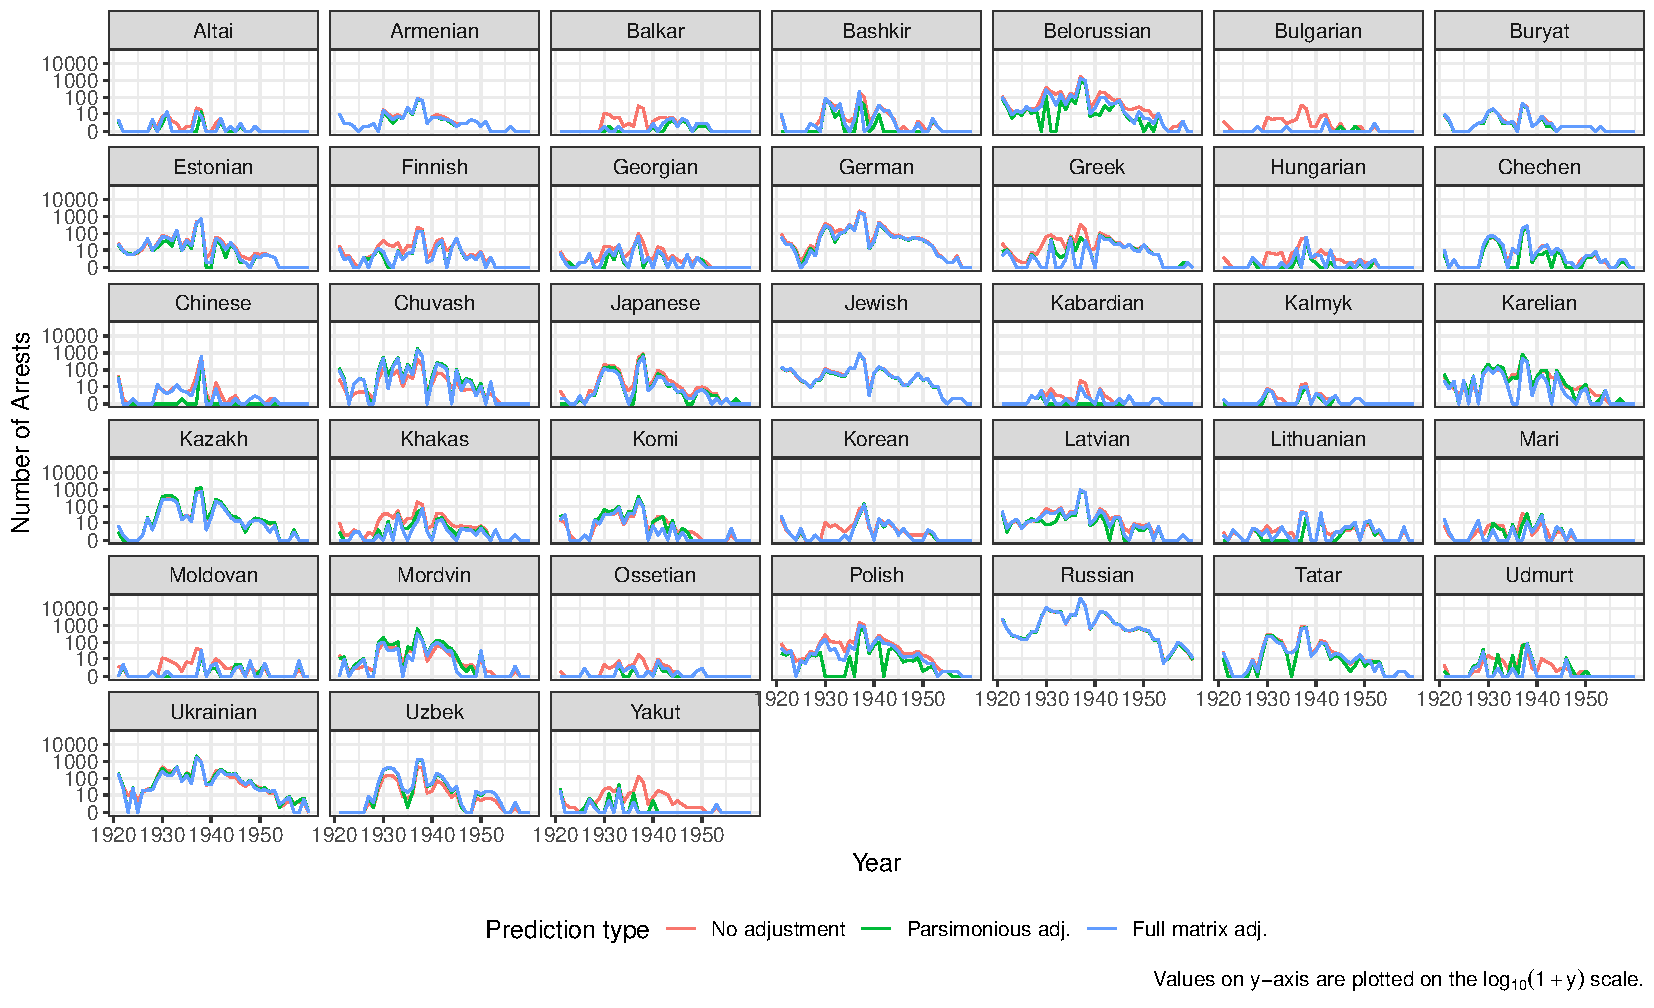
\includegraphics[width=1.2\textwidth]{plots/arrests/prediction_type_by_year.pdf}
\caption{Number of Predicted Arrests by Ethnicity, Year, and Prediction Adjustment}
\label{fig:prediction_type_by_year}
\end{figure}

\begin{figure}[!h]
\centering
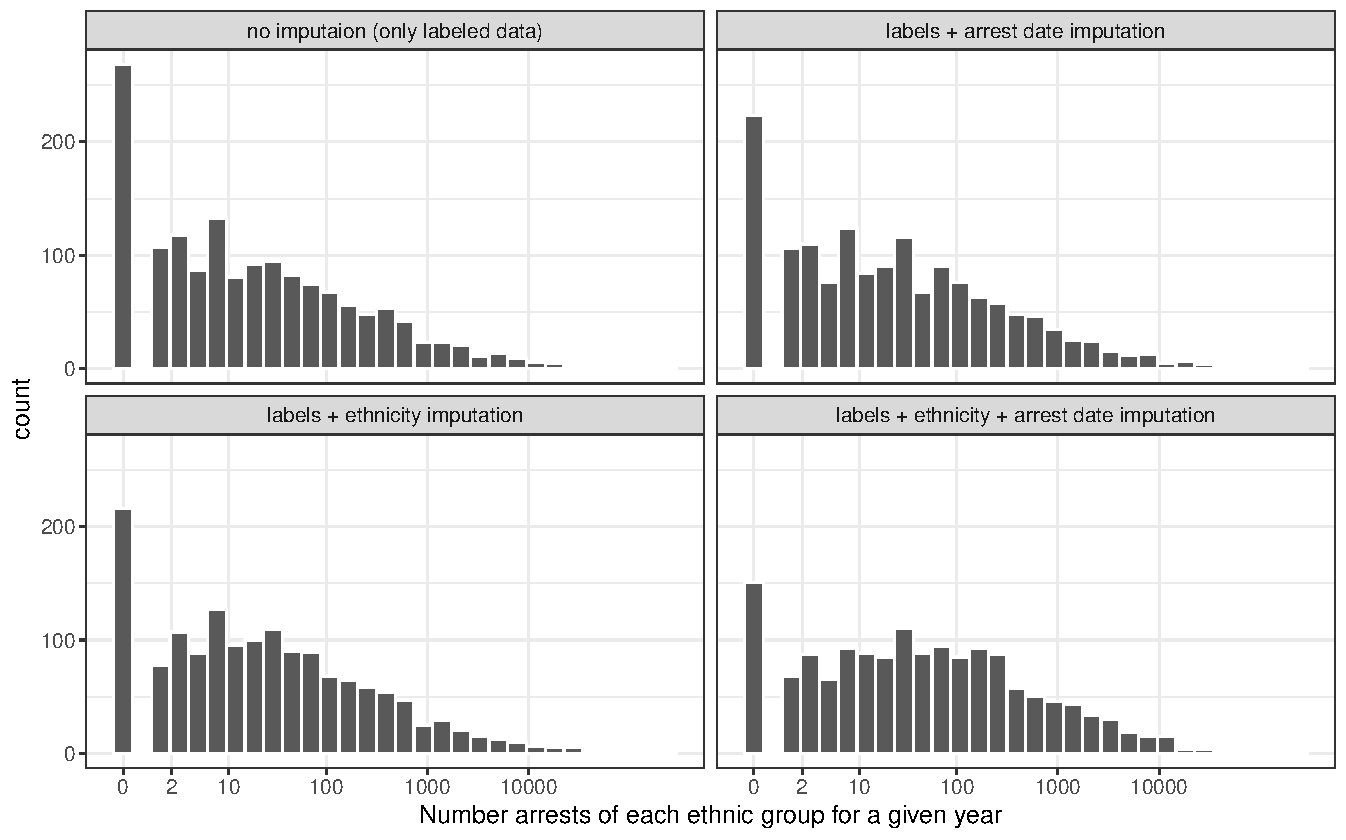
\includegraphics[width=1.2\textwidth]{plots/arrests/facet_hist.pdf}
\caption{Histograms of Arrests by Ethnicity and Year}
\label{fig:facet_by_year}
\end{figure}

\begin{figure}[!h]
\centering
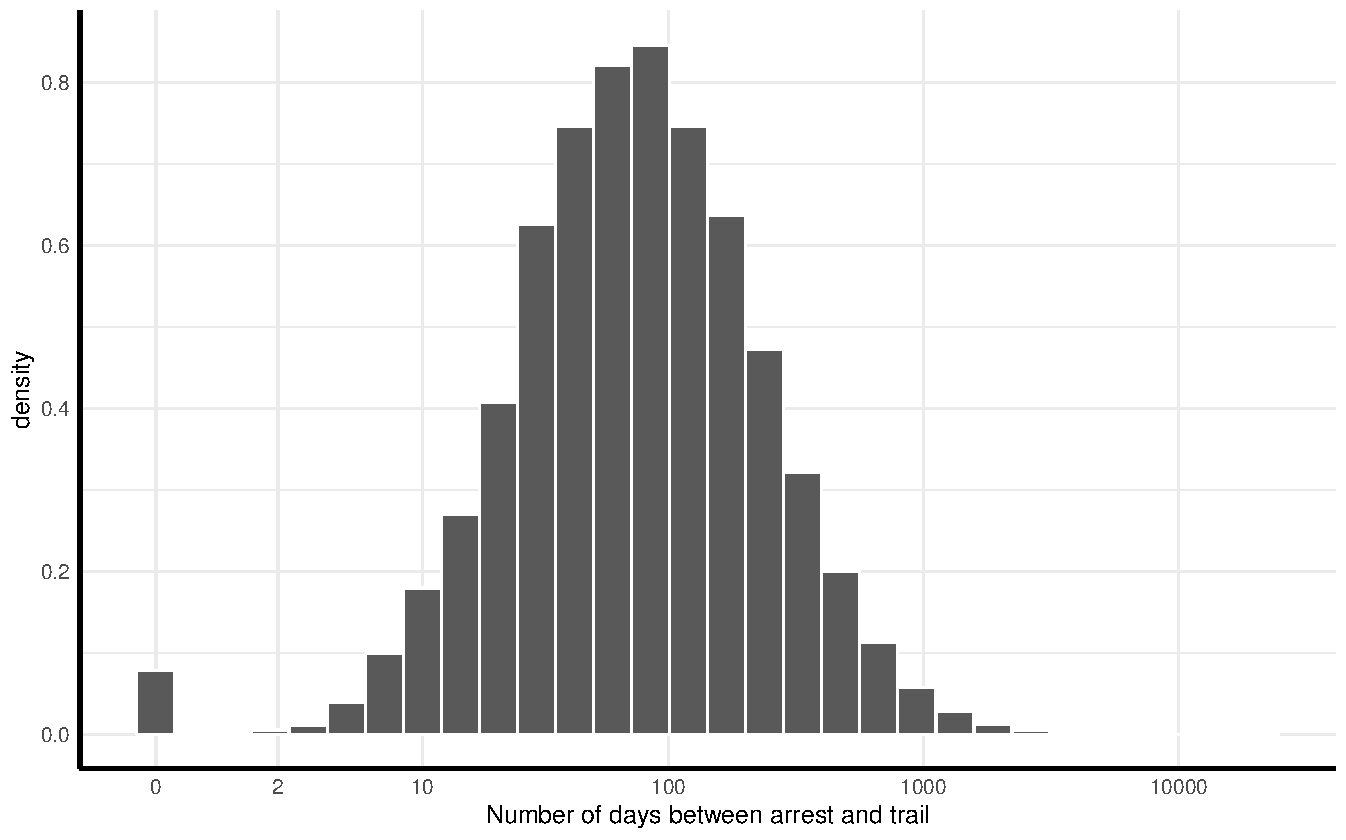
\includegraphics[width=1.2\textwidth]{plots/imputing_arrest_date/mixed_model_preds_hist.pdf}
\caption{Histogram of Imputed Number of Days between Arrest and Process}
\label{fig:mixed_model_preds_hist}
\end{figure}
\begin{figure}[!h]
\centering
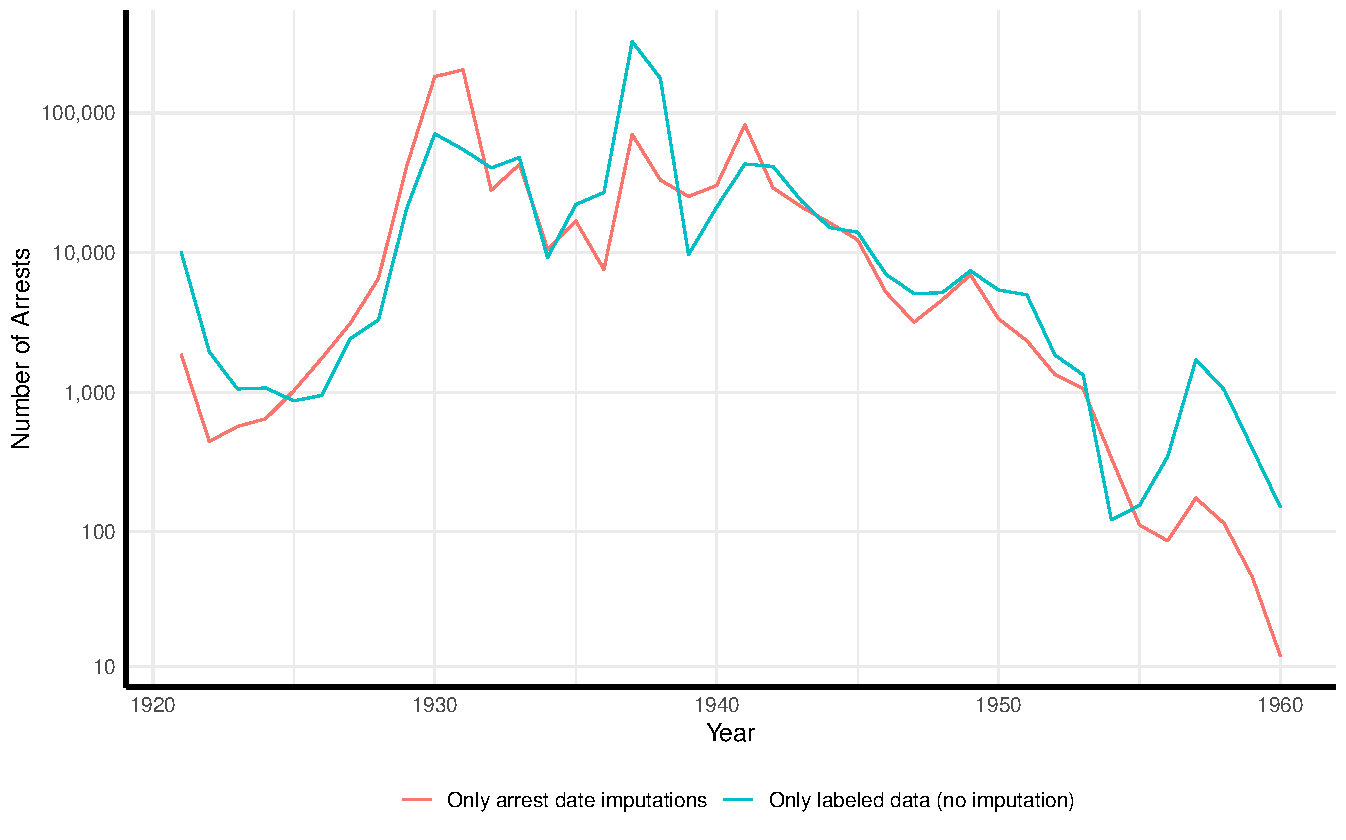
\includegraphics[width=1.2\textwidth]{plots/arrests/date_imputation_line.pdf}
\caption{Time Series of Arrests }
\label{fig:date_imputation_line}
\end{figure}

%
% Table created by stargazer v.5.2.2 by Marek Hlavac, Harvard University. E-mail: hlavac at fas.harvard.edu
% Date and time: p�, led 11, 2019 - 10:10:43
\begin{table}[!htbp] \centering 
  \caption{Difference-in-differences results} 
  \label{dif_table} 
\begin{tabular}{@{\extracolsep{5pt}}lcccc} 
\\[-1.8ex]\hline 
\hline \\[-1.8ex] 
 & \multicolumn{4}{c}{\textit{Dependent variable:}} \\ 
\cline{2-5} 
\\[-1.8ex] & \multicolumn{3}{c}{$\log(1 + y_{it})$} & $y_{it}$ \\ 
 & 1921-1958 & 1921-1945 & 1921-1945 & 1921-1958 \\ 
\\[-1.8ex] & (1) & (2) & (3) & (4)\\ 
\hline \\[-1.8ex] 
 $german*post\_1930$ & 1.196 & 0.731 & 0.855 & 683.539 \\ 
  & (0.887) & (0.984) & (0.963) & (1,495.164) \\ 
  & & & & \\ 
 $german*post\_1931$ & $-$0.779 & $-$0.872 & $-$0.847 & $-$61.209 \\ 
  & (1.177) & (1.198) & (1.292) & (1,983.046) \\ 
  & & & & \\ 
 $german*post\_1932$ & $-$0.439 & $-$0.532 & $-$0.507 & 63.854 \\ 
  & (1.177) & (1.198) & (1.292) & (1,983.046) \\ 
  & & & & \\ 
 $german*post\_1933$ & 0.365 & 0.272 & 0.297 & 199.791 \\ 
  & (1.177) & (1.198) & (1.292) & (1,983.046) \\ 
  & & & & \\ 
 $german*post\_1934$ & 2.040$^{*}$ & 1.947 & 1.971 & 996.604 \\ 
  & (1.177) & (1.198) & (1.292) & (1,983.046) \\ 
  & & & & \\ 
 $german*post\_1935$ & $-$0.638 & $-$0.731 & $-$0.706 & 49.979 \\ 
  & (1.177) & (1.198) & (1.292) & (1,983.046) \\ 
  & & & & \\ 
 $german*post\_1936$ & $-$0.134 & $-$0.227 & $-$0.202 & 71.041 \\ 
  & (1.177) & (1.198) & (1.292) & (1,983.046) \\ 
  & & & & \\ 
 $german*post\_1937$ & $-$0.214 & $-$0.307 & $-$0.282 & 637.291 \\ 
  & (1.177) & (1.198) & (1.292) & (1,983.046) \\ 
  & & & & \\ 
 $german*post\_1938$ & 1.322 & 0.772 & 0.537 & 2,304.034 \\ 
  & (0.906) & (0.972) & (0.934) & (1,526.238) \\ 
  & & & & \\ 
\hline \\[-1.8ex] 
Year dummies & Yes & Yes & Yes & Yes \\ 
Ethnicity dummies & Yes & Yes & Yes & Yes \\ 
Ethnicity time trends & Yes & Yes & No & Yes \\ 
Observations & 663 & 425 & 663 & 663 \\ 
R$^{2}$ & 0.890 & 0.900 & 0.864 & 0.428 \\ 
Adjusted R$^{2}$ & 0.875 & 0.882 & 0.850 & 0.350 \\ 
\hline 
\hline \\[-1.8ex] 
\textit{Note:}  & \multicolumn{4}{r}{$^{*}$p$<$0.1; $^{**}$p$<$0.05; $^{***}$p$<$0.01} \\ 
\end{tabular} 
\end{table} 

%\thispagestyle{empty}
 %this just pastes here the content of "appendix.tex" during LaTeX/PDF LaTeX/PDF TeXify translatation
\end{document}
